% concatenated from main.tex, macros.tex, plot.tex
% This is samplepaper.tex, a sample chapter demonstrating the
% LLNCS macro package for Springer Computer Science proceedings;
% Version 2.21 of 2022/01/12
%
\documentclass[runningheads,orivec]{llncs}
%
\usepackage[T1]{fontenc}
% T1 fonts will be used to generate the final print and online PDFs,
% so please use T1 fonts in your manuscript whenever possible.
% Other font encondings may result in incorrect characters.
%
\usepackage{graphicx}
% Used for displaying a sample figure. If possible, figure files should
% be included in EPS format.
%
% If you use the hyperref package, please uncomment the following two lines
% to display URLs in blue roman font according to Springer's eBook style:
% \usepackage{color}
% \renewcommand\UrlFont{\color{blue}\rmfamily}
%\urlstyle{rm}
%
\usepackage{amsmath}
\usepackage{amsfonts}
\usepackage{mathtools}
\usepackage{enumitem}
\usepackage{booktabs}
\usepackage{multirow}
\usepackage{tikz}

\setlist[enumerate,1]{label=(\roman*)}
\setlist{nolistsep}

\newcommand{\boxxx}[1]{%
  \smallskip
  \begin{center}
    \fbox{%
      \begin{minipage}{0.95\textwidth}#1\smallskip\end{minipage}%
    }%
  \end{center}%
  \smallskip
}

\newenvironment{ProofSketch}{%
  \renewcommand{\proofname}{Proof Sketch}\proof}{\endproof}

\usepackage{cite}            
\usepackage[colorlinks,
            citecolor=blue,
            urlcolor=blue,
            linkcolor=blue]{hyperref} % should always be the last package

\newif\ifIPCOFlag
\IPCOFlagtrue
\IPCOFlagfalse

\newcommand{\IPCO}[2]{\ifIPCOFlag#1\else#2\fi}

% \ifIPCO \else \fi can be used to switch the content.
% \ifIPCO
% This is the IPCO version.
% \else
% This if an arxiv version.
% \fi

\newcommand{\Rev}[1]{\textcolor{magenta}{#1}}
% \newcommand{\rev}[1]{#1}
\newcommand{\RevEnv}[1]{\begingroup\color{magenta}#1\endgroup}

\newcommand{\Comment}[1]{\marginpar{\small\textcolor{magenta}{#1}}}

\newenvironment{Review}
  {\par\vspace{0.3cm} % Add 2cm space before, forcing new paragraph
    \color{gray}\small
  }
  {
  } 

\newenvironment{Reply}
  {
  \noindent\small
  }
  {
  } 

\newcommand{\EtAl}{\textit{et al.}}

% \newcommand{\MacroColor}[1]{\textcolor{magenta}{#1}}
\newcommand{\MacroColor}[1]{#1}
\newcommand{\MacroColorTwo}[1]{#1}
% \newcommand{\MacroColorTwo}[1]{\textcolor{magenta}{#1}}

\newcommand{\MyQED}{\mbox{}\hfill$\square$}

\DeclareMathOperator*{\lexmin}{\MacroColor{lexmin}}
\DeclareMathOperator*{\lexmax}{\MacroColor{lexmax}}
\DeclareMathOperator*{\Argmin}{\MacroColor{argmin}}
\DeclareMathOperator*{\Argmax}{\MacroColor{argmin}}
\DeclareMathOperator*{\Arglexmin}{\MacroColor{arglexmin}}
\DeclareMathOperator*{\Arglexmax}{\MacroColor{arglexmin}}

\newcommand{\Size}[1]{\langle#1\rangle}
\newcommand{\SizeTwo}[2]{\langle#1,#2\rangle}
\newcommand{\SizeThree}[3]{\langle#1,#2,#3\rangle}
\newcommand{\SizeFour}[4]{\langle#1,#2,#3,#4\rangle}
\newcommand{\SizeFive}[5]{\langle#1,#2,#3,#4,#5\rangle}

\newcommand{\ZeroVector}{\mathbf{0}}
\newcommand{\OneVector}{\mathbf{1}}

\newcommand{\ComplexityClassStyle}[1]{#1}

\newcommand{\ClassP}{\MacroColor{\text{\ComplexityClassStyle{P}}}}
\newcommand{\ClassNP}{\MacroColor{\text{\ComplexityClassStyle{NP}}}}
\newcommand{\ClassCoNP}{\MacroColor{\text{\ComplexityClassStyle{coNP}}}}

\newcommand{\ThreeSAT}{\MacroColor{\textsc{3-SAT}}}
\newcommand{\BLPWithSingleUpperLevelVariable}{\MacroColor{$\textsc{BLP}_{\textsc{single}}$}}
\newcommand{\ValueOfBLPWithSingleUpperLevelVariableName}{\MacroColor{$\textsc{Val}_{\textsc{single}}$}}

\newcommand{\GlobalOptimalProblemName}{\MacroColor{$\textsc{Recog}_{\textsc{single}}^{\textsc{global}}$}}
\newcommand{\CompGlobalOptimalProblemName}{\MacroColor{$\overline{\textsc{Recog}}_{\textsc{single}}^{\textsc{global}}$}}

\newcommand{\LocalOptimalSearchName}{\MacroColor{$\textsc{Search}_{\textsc{single}}^{\textsc{local}}$}}

\newcommand{\ValueOfBLPWithSingleUpperLevelVariable}{\hyperref[ValueOfBLPWithSingleUpperLevelVariableAnchor]{\ValueOfBLPWithSingleUpperLevelVariableName{}}}

\newcommand{\GlobalOptimalProblem}{\hyperref[GlobalOptimalProblemAnchor]{\GlobalOptimalProblemName{}}}

\newcommand{\CompGlobalOptimalProblem}{\hyperref[GlobalOptimalProblemAnchor]{\CompGlobalOptimalProblemName{}}}

\newcommand{\OptimizationSense}{\MacroColor{\min}}
\newcommand{\TopLevelOptimizationSense}{\MacroColor{\inf}}
\newcommand{\MinusSignIfMinimization}{\MacroColor{-}}
\newcommand{\SignOfObjectiveSense}{\MacroColor{-}}
\newcommand{\OptimizationDualSense}{\MacroColor{\max}}
\newcommand{\ConstraintSense}{\MacroColor{\ge}}
\newcommand{\StrictConstraintSense}{\MacroColor{>}}
\newcommand{\ObjectiveImproveDirection}{\MacroColor{\le}}
\newcommand{\ObjectiveStrictImproveDirection}{\MacroColor{<}}
\newcommand{\ObjectiveImpairDirection}{\MacroColor{\ge}}
\newcommand{\ObjectiveStrictImpairDirection}{\MacroColor{>}}

\newcommand{\NVariables}{\MacroColor{n}}
\newcommand{\NConstraints}{\MacroColor{m}}
\newcommand{\IPNVariables}{\MacroColor{r}}

\newcommand{\OptValFunc}{\MacroColor{v}}
\newcommand{\OptSolSet}{\MacroColor{\mathcal{S}}}
\newcommand{\FeasSolSet}{\MacroColor{\mathcal{F}}}
\newcommand{\PartialOptValFunc}{\MacroColor{\psi}}

\newcommand{\SATBooleanFormula}{\MacroColor{F}}
\newcommand{\SATTruthAssignment}{\MacroColor{u}}
\newcommand{\SATReformulationBinaryVariable}{\MacroColor{x}}
\newcommand{\MaxElement}{\MacroColor{\sigma}}
\newcommand{\SolutionSizeEstimate}{\MacroColor{f_{\mathrm{sol}}}}
\newcommand{\SolutionSizeEstimateValue}{\MacroColor{\phi^{\text{norm}}}}

\newcommand{\ReformZ}{\MacroColor{z}}
\newcommand{\ReformFrac}{\MacroColor{w}}
\newcommand{\ReformAugFrac}{\MacroColor{f}}
\newcommand{\ReformPen}{\MacroColor{e}}
\newcommand{\LexUVar}{\MacroColor{\theta}}
\newcommand{\LexUVarSet}{\MacroColor{\Theta}}
\newcommand{\LexLVarS}{\MacroColor{s}}
\newcommand{\LexLVarT}{\MacroColor{t}}
\newcommand{\LexLVarU}{\MacroColor{u}}
\newcommand{\LexLVarV}{\MacroColor{v}}
\newcommand{\LexLVar}{\MacroColor{\eta}}
\newcommand{\LexLVarFuncU}{\MacroColor{f^u}}
\newcommand{\LexLVarFuncV}{\MacroColor{f^v}}
\newcommand{\LexLVarFuncZ}{\MacroColor{f^z}}
\newcommand{\LexLVarFuncInput}{\MacroColor{\theta}}
\newcommand{\LexWeight}{\MacroColor{p_{\mathrm{lex}}}}

\newcommand{\PenaltyThresholdFunction}{\MacroColor{p_{\mathrm{pen}}}}

\newcommand{\LemmaPenatyReformulationThreshold}{\MacroColor{M_{\mathrm{pen}}}}

\newcommand{\BinaryVector}{\MacroColor{\mu}}
\newcommand{\LexWeightValue}{\MacroColor{16}}

\newcommand{\UEncodingSize}{Size}
\newcommand{\UEncodingSizes}{Sizes}
\newcommand{\EncodingSize}{size}
\newcommand{\EncodingSizes}{sizes}

\begin{document}


% \title{Complexity of Bilevel Linear Programming\\with a Single Upper-Level Variable}
% \titlerunning{Complexity of Bilevel LP with a Single Upper-Level Variable}
% \author{Anonymous Author(s)}
% \institute{Anonymous Institute(s)}
% \authorrunning{Anonymous}
% \titlerunning{Anonymous Submission}

\title{Complexity of Bilevel Linear Programming\\with a Single Upper-Level Variable}
%
\titlerunning{Complexity of Bilevel LP with a Single Upper-Level Variable}
% If the paper title is too long for the running head, you can set
% an abbreviated paper title here

\author{Nagisa Sugishita\inst{1} \and
Margarida Carvalho\inst{2}}
%
% \authorrunning{F. Author et al.}
% First names are abbreviated in the running head.
% If there are more than two authors, 'et al.' is used.
%
\institute{Département de sciences de la décision, HEC Montréal
% \email{nagisa.sugishita@hec.ca}
\and
Département d'informatique et de recherche opérationnelle, Université de Montréal}
%


\maketitle              % typeset the header of the contribution
%
\begin{abstract}
Bilevel linear programming (LP) is one of the simplest classes of bilevel optimization problems, yet it is known to be \ClassNP{}-hard in general. Specifically, determining whether the optimal objective value of a bilevel LP is at least as good as a given threshold, a standard decision version of the problem, is \ClassNP{}-complete. However, this decision problem becomes tractable when either the number of lower-level variables or the number of lower-level constraints is fixed, which prompts the question: What if restrictions are placed on the upper-level problem? In this paper, we address this gap by showing that the decision version of bilevel LP remains \ClassNP{}-complete even when there is only a single upper-level variable, no upper-level constraints (apart from the constraint enforcing optimality of the lower-level decision) and all variables are bounded between 0 and 1. This result implies that fixing the number of variables or constraints in the upper-level problem alone does not lead to tractability in general. On the positive side, we show that there is a polynomial-time algorithm that finds a local optimal solution of such a rational bilevel LP instance. We also demonstrate that many combinatorial optimization problems, such as the knapsack problem and the traveling salesman problem, can be written as such a bilevel LP instance.
\keywords{Bilevel Programming \and Computational Complexity \and Lexicographic Linear Programming}
\end{abstract}
%
%
%

\section{Introduction}

Bilevel programming is a class of hierarchical optimization problems in which a \emph{leader} makes a decision first, and a \emph{follower} subsequently optimizes their own objective subject to the leader's choice. 
In this paper, we focus on the computational complexity of bilevel linear programming (LP), a setting where both the upper- and lower-level problems are LPs.
Unless stated otherwise, we consider the optimistic variant: when multiple optimal solutions exist for the follower, the one most favorable to the leader is chosen.
Even this simplest form of bilevel programming poses serious challenges in theory and practice.
A standard way to analyze the complexity of optimization problems is to consider their decision versions, specifically, determining whether the optimal objective value is equal to or less than a given threshold in a minimization problem.
Jeroslow~\cite{Jeroslow1985} was the first to show that the decision version of bilevel LP is \ClassNP{}-hard.
An alternative proof was given by Ben-Ayed and Blair~\cite{ben1990computational}.
Later, Hansen \EtAl{}~\cite{hansen1992new} showed that the problem remains \ClassNP{}-hard even when restricted to the min-max case.
More recently, Buchheim~\cite{Buchheim2023} proved its inclusion in \ClassNP{}, thereby establishing its \ClassNP{}-completeness.
Other decision problems have also been studied in the context of bilevel LP: Rodrigues \EtAl{}~\cite{RodriguesEtAl2024} showed that checking whether the problem is unbounded is \ClassNP{}-complete, and Vicente \EtAl{}~\cite{vicente1994descent} showed that recognizing local optimality of a given point is \ClassNP{}-hard.
Recently, Prokopyev and Ralphs~\cite{ProkopyevRalphs2024} studied the complexity of the search of a local optimal solution.

Given these negative complexity results, a natural line of research is to identify conditions under which bilevel LP becomes tractable. 
Such conditions can guide the design of efficient algorithms for practical instances.
For example, in the context of mixed-integer LP, a classical result by Lenstra Jr ~\cite{lenstra1983integer} establishes that problems with a fixed number of integer variables are solvable in polynomial time.
Similar results have been derived for bilevel LP.
Deng~\cite{deng1998complexity} demonstrated that bilevel LP is solvable in polynomial time when the number of lower-level variables is fixed.
Likewise, the arguments in~\cite{BasuEtAl2021} and~\cite{Buchheim2023} imply polynomial-time solvability when the number of lower-level constraints is fixed.
It was also shown that the toll pricing problem can be solved in polynomial time when the number of upper-level variables is fixed, enabling efficient algorithmic strategies~\cite{bui2024asymmetry}.
Related arguments and connections to a pessimistic variant of bilevel LP were very recently discussed in \cite{ketkov2025note}, released after the initial submission of this manuscript.

% A potential complication in bilevel problems arises from the presence of coupling (also known as linking) constraints in the upper-level problem, constraints that involve both upper- and lower-level variables.
% Notably, many of the known hardness results for bilevel LP hold even in the absence of coupling constraints.
% For example, the argument of~\cite{Jeroslow1985} implies that bilevel LP without coupling constraints remains \ClassNP{}-hard.
% Henke \EtAl{}~\cite{henke2025coupling} considered the use of the augmented Lagrangian to handle coupling constraints.
% % However, it is not evident whether this transformation can be carried out efficiently.

In this paper, we examine the decision version of bilevel LP under a particularly restricted setting: where there is only a single upper-level variable.
We show that even under this restricted structure, the decision problem remains \ClassNP{}-complete.
In particular, we prove a stronger result: bilevel LP is \ClassNP{}-complete even when there is only one upper-level variable and no upper-level constraints (other than the constraint enforcing the optimality of the lower-level variable with respect to the lower-level problem), and all variables are constrained to lie in the unit cube (i.e., when the lower-level constraints explicitly include bounds of 0 and 1 on each variable).
Our proof also establishes the \ClassNP{}-hardness of the decision version of the pessimistic formulation of bilevel LP. See the discussion following the proof of Theorem~\ref{theorem:ValueOfBLPWithSingleUpperLevelVariableIsNPHard} (page~\pageref{Rev:Pessimistic}) for details, including the definition of the pessimistic formulation.
We also prove that given a candidate solution, the problem of deciding whether it is optimal is also \ClassCoNP{}-complete.
On the positive side, we show that a locally optimal solution can be computed in polynomial time.
Furthermore, we show that many combinatorial problems, such as the knapsack problem and the traveling salesman problem, can be reformulated as bilevel LPs of this form, while preserving their optimal solutions.

\textbf{Paper Structure.}
This paper is organized as follows.
Section~\ref{sec:MainResult} formally introduces the class of bilevel LP instances, its decision version and its hardness, the main result of this paper.
Section~\ref{sec:AuxiliaryResults} presents auxiliary results that will be used to prove the main result in Section~\ref{sec:ProofOfTheorem1}.
Section~\ref{sec:ImplicationOfTheorem} discusses how combinatorial optimization problems can be transformed to bilevel LPs with a single upper-level variable, using the technique developed in the preceding sections.
Section~\ref{sec:ComplexityOfVerifyingASolution} is concerned with the complexity of searching for a globally and locally optimal solution.

\textbf{Conventions.}
We denote the binary encoding size of a rational number $p$ and a rational vector $v$ by $\Size{p}$ and $\Size{v}$, respectively.
Throughout the paper, we refer to the binary encoding size simply as the size.
For any sequence $a_1, \ldots, a_n$, we write $\Size{a_1, \ldots, a_n}$ to denote the sum $\Size{a_1} + \cdots + \Size{a_n}$.
We follow the encoding conventions described in~\cite{Schrijver1998}.
In particular, the size of a rational number $x = p/q$, where $p$ and $q$ are relatively prime integers, is given by $1 + \lceil \log_2(|p| + 1) \rceil + \lceil \log_2(|q| + 1) \rceil$.
We say that a vector, matrix, or optimization instance is \emph{rational} if and only if all its data are rational numbers.
Given an optimization instance $P$, we use $\OptValFunc(P)$, $\FeasSolSet(P)$, and $\OptSolSet(P)$ to denote the optimal objective value, the set of feasible solutions, and the set of optimal solutions, respectively.
We use $\ZeroVector$ (respectively, $\OneVector$) to denote the all-zeros (respectively, all-ones) vector, with the dimension clear from the context.
% To reduce clutter, we sometimes refer to column vectors inline.
% Given $u \in \mathbb{R}^{d_1}$ and $v \in \mathbb{R}^{d_2}$, we use the notation $(u, v)$ to denote the column vector
% $
% \begin{pmatrix} u \\ v \end{pmatrix} \in \mathbb{R}^{d_1 + d_2}.
% $

\section{Main Result}
\label{sec:MainResult}

In this paper, we study the hardness of rational bilevel LPs with a single upper-level variable.
In fact, we consider a more restrictive class where the upper-level problem has no constraints and all the variables are bounded to be within the unit cube.
Let \BLPWithSingleUpperLevelVariable{} denote the set of such bilevel LP instances.
An instance in \BLPWithSingleUpperLevelVariable{} can be written as:
\begin{align}
\min_{x_1, x_2} \ &
c_{2 1}^{\top} x_1 + c_{2 2} x_2
\tag{$\textsc{P}_{\textsc{single}}$}
\label{eq:NotationBLP}
\\
\text{s.t.} \
&
x_1 \in \Argmin_{x_1'} \{ c_{1 1}^{\top} x_1' : A_{1 1} x_1' + A_{1 2} x_2 \ge b_1,
\ZeroVector \le x_1' \le \OneVector, 0 \le x_2 \le 1
\}, \notag
\end{align}
where $c_{1 1}, c_{2 1} \in \mathbb{Q}^{\NVariables}$, $c_{2 2} \in \mathbb{Q}$, $A_{1 1} \in \mathbb{Q}^{\NConstraints \times \NVariables}$, and $A_{1 2}, b_1 \in \mathbb{Q}^{\NConstraints}$.
A subtle remark is in order. Note that the lower-level constraints impose the bounds on the upper-level variable $x_2$.
If the leader chooses $x_2$ outside these bounds, the lower-level problem becomes infeasible, consequently resulting into a bilevel infeasible solution to \eqref{eq:NotationBLP}.
In other words, although the upper-level problem has no variable bounds on $x_2$, effective bounds are implicitly enforced by the lower-level constraints.

Consider the following decision problem:
\begin{align*}
& 
\parbox{0.75\textwidth}{Given a rational instance \eqref{eq:NotationBLP} and a rational 
number $k$, is the optimal objective value less than or equal to $k$?}
\label{ValueOfBLPWithSingleUpperLevelVariableAnchor}
\tag{\ValueOfBLPWithSingleUpperLevelVariable{}}
\end{align*}
We will prove the following result.

\begin{theorem}
\label{theorem:ValueOfBLPWithSingleUpperLevelVariableIsNPHard}
The decision problem \ValueOfBLPWithSingleUpperLevelVariable{} is \ClassNP{}-complete.
\end{theorem}

In Section~\ref{sec:ProofOfTheorem1}, we prove Theorem~\ref{theorem:ValueOfBLPWithSingleUpperLevelVariableIsNPHard}.
To this end, we provide a reduction from \ThreeSAT{} to \ValueOfBLPWithSingleUpperLevelVariable{}.
That is, given a Boolean formula $\SATBooleanFormula$ in 3-conjunctive normal form (3CNF), we construct a \BLPWithSingleUpperLevelVariable{} instance such that the optimal objective value is $-1$ if $\SATBooleanFormula$ is satisfiable and $0$ otherwise.

To simplify the exposition, we divide the reduction into several steps.
First, we construct a bilevel LP instance with multiple upper-level variables and upper-level constraints (instance~\ref{eq:SATBLPFirst}).
We then reduce the problem to a bilevel LP with a single upper-level variable (instance~\ref{eq:SATBilevelWeightedProblem}).
Lastly, we eliminate the upper-level constraints via a penalty method (instance~\ref{eq:SATBLPLast}).
The final instance is a bilevel LP with a single upper-level variable and no upper-level constraints.
We will show that the optimal objective value is preserved throughout these transformations.

To develop our argument, we need to analyse general bilevel LPs, i.e., instances with multiple variables and constraints in the upper-level problem.
Thus, in Section~\ref{sec:AuxiliaryResults}, we provide some auxiliary results to study general bilevel LPs.

\section{Auxiliary Results}
\label{sec:AuxiliaryResults}

This section presents auxiliary results that will be used in Section~\ref{sec:ProofOfTheorem1} to prove Theorem~\ref{theorem:ValueOfBLPWithSingleUpperLevelVariableIsNPHard}.
Section~\ref{subsec:EstimateOfOptimalSolutionSize} provides an estimate on the size of an optimal solution to a bilevel LP.
To the best of our knowledge, such bounds have not been explicitly discussed in the literature.
Section~\ref{subsec:ReformulationOfCouplingConstraints} presents a method for reformulating upper-level constraints as lower-level constraints.

\subsection{Estimate of Optimal Solution Size}
\label{subsec:EstimateOfOptimalSolutionSize}

We begin by presenting a bound on the size of an optimal solution to an LP, which will be used to estimate the size of solutions for bilevel LPs.
\begin{lemma}
\label{lemma:estimate-of-primal-linear-inequality}
Let $A, B \in \mathbb{Q}^{\NConstraints \times \NVariables}$, $a, b \in \mathbb{Q}^{\NConstraints}$, and $c \in \mathbb{Q}^{\NVariables}$.  
Let $\sigma$ denote the maximum \EncodingSize{} of the entries in $A$, $B$, $a$, and $b$.  
Consider the LP
\[
\min_{x} \left\{ c^{\top} x : A x \ConstraintSense a, B x \StrictConstraintSense b \right\}.
\]
If an optimal solution exists, then there exists a rational optimal solution $\bar{x}$ of size bounded by a polynomial in $\NVariables$ and $\sigma$.  
That is, there exists a polynomial $\SolutionSizeEstimate$ such that $\Size{\bar{x}} \le \SolutionSizeEstimate(\NVariables, \sigma)$.
\end{lemma}
Note that the optimization instance in Lemma~\ref{lemma:estimate-of-primal-linear-inequality} includes strict inequalities.
Nonetheless, we refer to such instances as LPs throughout this paper.
Strict inequalities are used later in the proof of Lemma~\ref{lemma:PenaltyReformulation}.
\phantomsection\label{Rev:MorePreciseReferenceToSchrijver}
For the proof, see Corollary~10.2 in~\cite{Schrijver1998} (the corollary only discusses weak inequalities, but the extension to strict inequalities is straightforward).
We are now ready to state an analogous result for bilevel LPs.
\begin{lemma}
\label{lemma:SolutionSizeEstimate}
Let
$A_{1 1} \in \mathbb{Q}^{\NConstraints_1 \times \NVariables_1}, A_{1 2} \in \mathbb{Q}^{\NConstraints_1 \times \NVariables_2}, A_{2 1} \in \mathbb{Q}^{\NConstraints_2 \times \NVariables_1}, A_{2 2} \in \mathbb{Q}^{\NConstraints_2 \times \NVariables_2}$, $b_1 \in \mathbb{Q}^{\NConstraints_1}, b_2 \in \mathbb{Q}^{\NConstraints_2}$, $c_{1 1}, c_{2 1} \in \mathbb{Q}^{\NVariables_1}$ and $c_{2 2} \in \mathbb{Q}^{\NVariables_2}$.
Let $\NVariables = \NVariables_1 + \NVariables_2$ and $\sigma$ denote the maximum \EncodingSize{} of the entries in $A_{1 1}, A_{1 2}, A_{2 1}, A_{2 2}$, $b_1$, and $b_2$.
Consider the bilevel LP
\begin{align}
\min_{x_1, x_2} \ &
c_{2 1}^{\top} x_1 + c_{2 2}^{\top} x_2
\label{eq:SolutionSizeEstimateBLP}
\\
\text{s.t.} \ &
A_{2 1} x_1 + A_{2 2} x_2 \ge b_2, \notag \\
&
x_1 \in \Argmin_{x_1'} \{ c_{1 1}^{\top} x_1' : A_{1 1} x_1' + A_{1 2} x_2 \ge b_1 \}. \notag
\end{align}
If an optimal solution exists, then there exists a rational optimal solution $(\bar{x}_1, \bar{x}_2)$ such that $\SizeTwo{\bar{x}_1}{\bar{x}_2} \le \SolutionSizeEstimate(\NVariables, \sigma)$, \phantomsection\label{Rev:DefOfFSol} where $\SolutionSizeEstimate$ is the polynomial defined in Lemma~\ref{lemma:estimate-of-primal-linear-inequality}.
\end{lemma}
The proof is given in \IPCO{the full version of the paper~\cite{sugishita2025complexitybilevellinearprogramming}}{Appendix~\ref{sec:proof_of_lemma_solution_size_estimate}}.
\phantomsection\label{Rev:RelationToBuchheim}%
We note that this is closely related to the result of~\cite{Buchheim2023}, where it is shown that the decision version of bilevel LP belongs to \ClassNP{}.
Their argument can be used to establish that, whenever the optimal objective value is below a given threshold, there exists a rational feasible solution of polynomial encoding length with objective value below the threshold. 
In contrast, Lemma~\ref{lemma:SolutionSizeEstimate} guarantees the existence of a rational optimal solution of polynomial encoding length, provided that an optimal solution exists.
% TODO Recall fsol is polynomial in Lemma 1.

\subsection{Reformulation of Upper-Level Constraints}
\label{subsec:ReformulationOfCouplingConstraints}

\phantomsection\label{Rev:ComplicationByCoupling}
If the upper-level problem has a constraint that does not involve any lower-level variables, it can be ``moved'' to the lower-level problem without changing the feasible solution set. 
However, if an upper-level constraint involves lower-level variables, special care must be taken. 
In this section, we present our approach for removing such constraints by introducing a penalty term in the objective.
Let
\begin{align}
\min_{x_1, x_2} \ &
c_{2 1}^{\top} x_1 + c_{2 2}^{\top} x_2 
\tag{$Q_{\mathrm{blp}}$}
\label{eq:PenaltyBefore}
\\
\text{s.t.} \ &
A_{2 1} x_1 + A_{2 2} x_2 \ge b_2, \notag \\
&
\bar{A}_{2 1} x_1 + \bar{A}_{2 2} x_2 \ge \bar{b}_2, \notag \\
&
x_1 \in \Argmin_{x_1'} \{ c_{1 1}^{\top} x_1' : A_{1 1} x_1' + A_{1 2} x_2 \ge b_1 \}, \notag 
\end{align}
where $A_{1 1} \in \mathbb{Q}^{\NConstraints_1 \times \NVariables_1}, A_{1 2} \in \mathbb{Q}^{\NConstraints_1 \times \NVariables_2}, A_{2 1} \in \mathbb{Q}^{\NConstraints_2 \times \NVariables_1}, A_{2 2} \in \mathbb{Q}^{\NConstraints_2 \times \NVariables_2}, \bar{A}_{2 1} \in \mathbb{Q}^{\NConstraints_2' \times \NVariables_1}, \bar{A}_{2 2} \in \mathbb{Q}^{\NConstraints_2' \times \NVariables_2}$, $b_1 \in \mathbb{Q}^{\NConstraints_1}, b_2 \in \mathbb{Q}^{\NConstraints_2}, \bar{b}_2 \in \mathbb{Q}^{\NConstraints_2'}$, $c_{1 1}, c_{2 1} \in \mathbb{Q}^{\NVariables_1}$ and $c_{2 2} \in \mathbb{Q}^{\NVariables_2}$.
We are interested in ``replacing'' constraints $\bar{A}_{2 1} x_1 + \bar{A}_{2 2} x_2 \ge \bar{b}_2$ in \eqref{eq:PenaltyBefore} with a penalty term in the objective with a help of a single variable $\ReformPen \in \mathbb{R}$ and a real number $M$:
\begin{align}
\min_{x_1, x_2, \ReformPen} \ &
c_{2 1}^{\top} x_1 + c_{2 2}^{\top} x_2 + M \ReformPen
\tag{$Q_{\mathrm{blp}}'(M)$}
\label{eq:PenaltyAfter}
\\
\text{s.t.} \ &
A_{2 1} x_1 + A_{2 2} x_2 \ge b_2, \notag \\
&
(x_1, \ReformPen) \in \Argmin_{x_1', \ReformPen'} 
\left\{ 
\begin{array}{rl}
&
A_{1 1} x_1' + A_{1 2} x_2 \ge b_1, \\
c_{1 1}^{\top} x_1' : 
&
\bar{A}_{2 1} x_1' + \bar{A}_{2 2} x_2 + \ReformPen' \OneVector \ge \bar{b}_2, \\
&
\ReformPen' \in I_{\ReformPen}
\end{array}
\right\}, \notag 
\end{align}
where $I_{\ReformPen}$ is $[0, 1]$ or $[0, \infty)$.
The following result holds for both choices of $I_{\ReformPen}$.
The former is more convenient for our purposes, as we would like all variables to be constrained within $[0, 1]$, whereas the latter is more natural in applications.
\begin{lemma}
\label{lemma:PenaltyReformulation}
Let $I_{\ReformPen}$ is $[0, 1]$ or $[0, \infty)$, and suppose \eqref{eq:PenaltyBefore} and \eqref{eq:PenaltyAfter} have an optimal solution for any $M > 0$.
Let $\NVariables = \NVariables_1 + \NVariables_2$, $\sigma$ denote the maximum \EncodingSize{} of entries in $A_{1 1}$, $A_{1 2}$, $A_{2 1}$, $A_{2 2}$, $\bar{A}_{2 1}$, $\bar{A}_{2 2}$, $b_1$, $b_2$, $\bar{b}_2$, and $c_{\infty} = \max\{ \| c_{2 1} \|_{\infty}, \| c_{2 2} \|_{\infty}, 1 \}$.
For any $M \ge 3 \NVariables c_{\infty} 4^{\SolutionSizeEstimate(\NVariables + 1, \sigma)}$, the following relations hold:
\begin{enumerate}
\item $\OptValFunc\eqref{eq:PenaltyBefore} = \OptValFunc\eqref{eq:PenaltyAfter}$;
\item $\OptSolSet\eqref{eq:PenaltyAfter} = \{(x_1, x_2, 0) : (x_1, x_2) \in \OptSolSet\eqref{eq:PenaltyBefore} \}$.
\end{enumerate}
\end{lemma}
\phantomsection\label{Rev:AugmentedLagrangian}
A related penalty-based reformulation appears in~\cite{henke2025coupling}, although it is unclear whether their transformation can be performed efficiently.
Recent works~\cite{henke2025couplingpessimistic,lefebvre2024exact} investigate this question.
In \IPCO{the full version of the paper~\cite{sugishita2025complexitybilevellinearprogramming}}{Appendix~\ref{sec:ProofOfLemmaPenaltyReformulation}}, we provide an alternative and simpler proof of Lemma~\ref{lemma:PenaltyReformulation}.

\section{Proof of Theorem~\ref{theorem:ValueOfBLPWithSingleUpperLevelVariableIsNPHard}}
\label{sec:ProofOfTheorem1}

We begin by constructing a bilevel LP instance with multiple upper-level variables.
Let \( F \) be a Boolean formula in 3CNF with \( n \) variables \( \SATTruthAssignment{}_1, \ldots, \SATTruthAssignment{}_n \) and \( p \) clauses.
Following \cite{marcotte2005bilevel,pardalos1988checking}, \( F \) can be represented by a system of linear inequalities over binary variables:
$
A_{\SATBooleanFormula} \SATReformulationBinaryVariable{} \geq \OneVector - a_{\SATBooleanFormula}, \ \SATReformulationBinaryVariable{} \in \{0,1\}^n,
$
where \( A_{\SATBooleanFormula} \in \mathbb{Z}^{p \times n} \), \( a_{\SATBooleanFormula} \in \mathbb{Z}^p \).
A satisfying truth assignment corresponds exactly to a feasible solution, where $u_i = \text{true}$ corresponds to $x_i = 1$.
The inequalities are constructed clause by clause. For a clause $(l_1 \vee l_2 \vee l_3)$, we add the inequality 
\[
\sum_{i: u_i \in \{l_1, l_2, l_3\}} x_i
+
\sum_{i: \neg u_i \in \{l_1, l_2, l_3\}} (1 - x_i)
\ge 1.
\]
For example,
$
F = (\SATTruthAssignment{}_1 \vee \neg \SATTruthAssignment{}_2) \wedge (\neg \SATTruthAssignment{}_1 \vee \neg \SATTruthAssignment{}_2 \vee \SATTruthAssignment{}_3)
$
corresponds to
\[
\SATReformulationBinaryVariable{}_1 + (1 - \SATReformulationBinaryVariable{}_2) \geq 1, \quad (1 - \SATReformulationBinaryVariable{}_1) + (1 - \SATReformulationBinaryVariable{}_2) + \SATReformulationBinaryVariable{}_3 \geq 1, \quad \SATReformulationBinaryVariable{} \in \{0,1\}^3.
\]
% First, $A_{\SATBooleanFormula}$ and $a_{\SATBooleanFormula}$ are set to $0$.
% Then, we scan the clauses one by one.
% A positive literal \( \SATTruthAssignment{}_i \) in the \( j \)-th clause increments the \((j,i)\) element of \( A_{\SATBooleanFormula} \) by 1, while a negated literal \(\neg \SATTruthAssignment{}_i\) decrements the \((j,i)\) element of \( A_{\SATBooleanFormula} \) and increments the $j$-th element of \( a_{\SATBooleanFormula} \).
% For example,
% $
% F = (\SATTruthAssignment{}_1 \vee \neg \SATTruthAssignment{}_2) \wedge (\neg \SATTruthAssignment{}_1 \vee \neg \SATTruthAssignment{}_2 \vee \SATTruthAssignment{}_3)
% $
% corresponds to
% \[
% A_{\SATBooleanFormula} = \begin{pmatrix} 1 & -1 & 0 \\ -1 & -1 & 1 \end{pmatrix}, \quad
% a_{\SATBooleanFormula} = \begin{pmatrix} 1 \\ 2 \end{pmatrix},
% \]
% yielding inequalities
% \[
% \SATReformulationBinaryVariable{}_1 + (1 - \SATReformulationBinaryVariable{}_2) \geq 1, \quad (1 - \SATReformulationBinaryVariable{}_1) + (1 - \SATReformulationBinaryVariable{}_2) + \SATReformulationBinaryVariable{}_3 \geq 1, \quad \SATReformulationBinaryVariable{} \in \{0,1\}^3.
% \]
In the following, we say that a binary vector satisfies \( \SATBooleanFormula \) if and only if the corresponding truth assignment satisfies \( \SATBooleanFormula \).

Now, consider the following bilevel LP instance:
\begin{alignat}{2}
\min_{x, y, \ReformFrac} \ & 2 \sum_{i = 1}^{n} \left(y - 2 \ReformFrac_i \right) - \frac{2}{n} \sum_{i = 1}^n \ReformFrac_i
\tag{P${}_{\text{3SAT}}^{\text{}}(\SATBooleanFormula)$}
\label{eq:SATBLPFirst}
\\
\text{s.t.} \ &
A_{\SATBooleanFormula} x \ge \left(\frac{3}{2} - \frac{1}{2} y\right) \OneVector - a_{\SATBooleanFormula}, \label{eq:SATBLPFirstConstraintOne} \\
&
\frac{1}{2} - \frac{1}{2} y \le x_{i} \le \frac{1}{2} + \frac{1}{2} y, 
&&
\forall i = 1, \ldots, \NVariables,
\label{eq:SATBLPFirstConstraintTwo} \\
& 0 \le x_i \le 1, \ 0 \le y \le 1, 
&&
\forall i = 1, \ldots, \NVariables, 
\hspace{13em}
\notag \\
&
\mathmakebox[0cm][l]{
\ReformFrac \in \Argmin_{\ReformFrac'} 
\left\{ 
\sum_{i = 1}^n \ReformFrac_i'
:
-\ReformFrac_i' \le x_i - 1/2 \le \ReformFrac_i', 0 \le \ReformFrac_i' \le 1, \ i = 1, \ldots, n
\right\}. 
}
\notag 
\end{alignat}
\phantomsection\label{Rev:MeaningOfLowerLevel} The lower-level problem measures the closeness of the upper-level decision variable $x$ to the nearest integers by setting $\ReformFrac_i = |x_i - 1/2|$, which is maximized when $x_i \in \{0, 1\}$.
This instance is obtained from the one studied by Vicente \EtAl{}~\cite{vicente1994descent} (see also \cite{RodriguesEtAl2024}).
Instance \eqref{eq:SATBLPFirst} differs from their instance in that we removed some redundant variables from the lower-level problem for simplification and added variable bounds $0 \le x_i \le 1$, $0 \le y \le 1$ and $0 \le w_i \le 1$ for each $i = 1, \ldots, \NVariables$.
Without the variable bounds, the instance is unbounded if and only if $\SATBooleanFormula$ is satisfiable.
In our case (i.e., with the variable bounds), the optimal objective value of \eqref{eq:SATBLPFirst} is $-1$ if $\SATBooleanFormula$ is satisfiable and 0 otherwise, as stated below.
\begin{lemma}
\label{lemma:SATBLPFirst}
\mbox{}
\begin{enumerate}
\item
Suppose $\SATBooleanFormula$ is unsatisfiable.
Then, $x_i = 1/2$ for $i = 1, \ldots, \NVariables$, $y = 0$, and $w = \ZeroVector$ is optimal for \eqref{eq:SATBLPFirst} and $\OptValFunc\eqref{eq:SATBLPFirst} = 0$.
\item
Suppose $\SATBooleanFormula$ is satisfiable and let $\BinaryVector$ be a binary vector satisfying $\SATBooleanFormula$.
Then, $x = \BinaryVector$, $y = 1$, and $w = \ZeroVector$  is optimal for \eqref{eq:SATBLPFirst} and $\OptValFunc\eqref{eq:SATBLPFirst} = -1$.
\end{enumerate}
\end{lemma}
See \IPCO{the full version of the paper~\cite{sugishita2025complexitybilevellinearprogramming}}{Appendix~\ref{sec:proof_of_lemma_sat_multivariate_blp_formulation}} for the proof.

To simplify the notation in the following argument, we write $\ReformZ = (x, y) \in \mathbb{R}^{\NVariables + 1}$ and the constraints~\eqref{eq:SATBLPFirstConstraintOne} and~\eqref{eq:SATBLPFirstConstraintTwo} as $B_{\SATBooleanFormula} \ReformZ \ge b_{\SATBooleanFormula}$.
Furthermore, we introduce $\ReformAugFrac \in \mathbb{R}^{\NVariables + 1}$ such that $\ReformAugFrac_i = |\ReformZ_i - 1/2|$ for $i = 1, \ldots, \NVariables + 1$.
With this notation, \eqref{eq:SATBLPFirst} can be written as
\begin{align}
\min_{\ReformZ, \ReformAugFrac} \ & 2 \sum_{i = 1}^{n} \left(\ReformZ_{\NVariables + 1} - 2 \ReformAugFrac_i \right) - \frac{2}{n} \sum_{i = 1}^{\NVariables} \ReformAugFrac_i
\tag{P${}_{\text{mult}}^{\text{}}(\SATBooleanFormula)$}
\label{eq:SATBLPMultVariables}
\\
\text{s.t.} \ &
B_{\SATBooleanFormula} \ReformZ \ge b_{\SATBooleanFormula}, \
0 \le \ReformZ_i \le 1, \
\forall i = 1, \ldots, \NVariables + 1, 
\notag 
\\
&
\ReformAugFrac \in \Argmin_{\ReformAugFrac'} 
\left\{ 
\sum_{i = 1}^{\NVariables + 1} \ReformAugFrac_i'
:
\begin{array}{l}
-\ReformAugFrac_i' \le z_i - 1/2 \le \ReformAugFrac_i', 0 \le \ReformAugFrac_i' \le 1, \ i = 1, \ldots, \NVariables + 1
\end{array}
\right\}. \notag 
\end{align}
The formulation \eqref{eq:SATBLPMultVariables} differs from \eqref{eq:SATBLPFirst} by the inclusion of an additional variable, $\ReformAugFrac_{\NVariables + 1}$.  
Nonetheless, both problems attain the same optimal objective value.  
The additional variable is introduced purely for notational convenience in the analysis that follows.

Now, we use a lexicographic LP to replace the upper-level variables $\ReformZ$ in \eqref{eq:SATBLPMultVariables} with a single upper-level variable $\LexUVar$.
Consider
\begin{align}
\min_{\LexUVar, \ReformZ, \ReformAugFrac, \LexLVarS, \LexLVarT, \LexLVarU} \ & 2 \sum_{i = 1}^{n} \left(\ReformZ_{\NVariables + 1} - 2 \ReformAugFrac_i \right) - \frac{2}{n} \sum_{i = 1}^n \ReformAugFrac_i
\tag{P${}_{\text{lex}}^{\text{}}(\SATBooleanFormula)$}
\label{eq:SATBilevelLexProgramming}
\\
\text{s.t.} \ &
B_{\SATBooleanFormula} \ReformZ \ge b_{\SATBooleanFormula},
0 \le \LexUVar \le 1, \notag \\
&
(\ReformZ, \ReformAugFrac, \LexLVarS, \LexLVarT, \LexLVarU) 
\in
\OptSolSet\eqref{eq:SATBilevelLexProgrammingLowerLevel},
\notag 
\end{align}
where
\begin{alignat}{3}
\lexmin_{\ReformZ, \ReformAugFrac, \LexLVarS, \LexLVarT, \LexLVarU} \ & 
\mathmakebox[0cm][l]{
\left\{
\LexLVarS_{\NVariables + 1} + \LexLVarT_{\NVariables + 1}, \
\ldots, \
\LexLVarS_{1} + \LexLVarT_{1}, \
\sum_{i = 1}^{\NVariables + 1} \ReformAugFrac_i
\right\}
}
\tag{P${}_{\text{lex}}^{\text{low}}(\NVariables + 1, \LexUVar)$}
\label{eq:SATBilevelLexProgrammingLowerLevel}
\\
% ------------------------------------------------------------
\text{s.t.} \
&
\LexLVarU_{\NVariables + 1} = \theta,
\notag
\\
&
\LexLVarS_i \ge (3/2) \LexLVarU_{i} - 1/2,
\qquad
&&
\LexLVarT_i \ge (3/2) \LexLVarU_{i} - 1,
\qquad
&&
\forall i = 1, \ldots, \NVariables + 1,
\notag \\
&
z_i = 2 (\LexLVarS_i - \LexLVarT_i),
&&
-\ReformAugFrac_i \le z_i - 1/2 \le \ReformAugFrac_i, 
\quad
&&
\forall i = 1, \ldots, \NVariables + 1,
\notag \\
% --------------------------------------------
&
\LexLVarU_{i - 1} = 3 \LexLVarU_i - 2 z_i,
&&
&&
\forall i = 2, \ldots, \NVariables + 1, \notag \\
&
0 \le \ReformZ_i, \ReformAugFrac_i, \LexLVarS_i, \LexLVarT_i, \LexLVarU_i \le 1,
&&
&&
\forall i = 1, \ldots, \NVariables + 1,
\notag
\end{alignat}
with $\LexUVar \in \mathbb{R}$, $\ReformZ, \ReformAugFrac, \LexLVarS, \LexLVarT, \LexLVarU \in \mathbb{R}^{\NVariables + 1}$.
\phantomsection\label{Rev:Lexmin} Here, $\lexmin$ denotes the lexicographic minimization: the first objective is given highest priority, and later objectives are considered only when earlier ones are equal.
In~\eqref{eq:SATBilevelLexProgramming}, $\ReformZ$ denotes a lower-level variable. We intentionally use the same symbol $\ReformZ$, for reasons that will be clarified later.
For each $\theta \in [0, 1]$, \eqref{eq:SATBilevelLexProgrammingLowerLevel} has a unique solution, and can be solved analytically, as stated below.
\begin{lemma}
\label{lemma:LexLowerLevelSolution}
\mbox{}
\begin{enumerate}
\item 
\label{lemma:LexLowerLevelSolutionAssertionOne}
For any $\LexUVar \in [0, 1]$, it holds that
\begin{align*}
&
\OptSolSet\eqref{eq:SATBilevelLexProgrammingLowerLevel} =
\\
&
\
\left\{
\begin{pmatrix}
\ReformZ \\ \ReformAugFrac \\ \LexLVarS \\ \LexLVarT \\ \LexLVarU
\end{pmatrix}
:
\begin{array}{llllll}
&
\LexLVarU_{\NVariables + 1} = \theta,
\notag
\\
&
\LexLVarS_i = [(3/2) \LexLVarU_i - 1/2]^+, 
\quad
&&
\LexLVarT_i = [(3/2) \LexLVarU_i - 1]^+,
\quad
&&
\forall i = 1, \ldots, \NVariables + 1,
\\
&
z_i = \LexLVarFuncZ(\LexLVarU_{i}),
&&
\ReformAugFrac_i = |z_i - 1/2|,
&&
\forall i = 1, \ldots, \NVariables + 1,
\\
% --------------------------------------------
&
\LexLVarU_{i - 1} = \LexLVarFuncU(\LexLVarU_i),
&&
&&
\forall i = 2, \ldots, \NVariables + 1, \notag 
\notag 
\end{array}
\right\},
\end{align*}
where $[ a ]^+ = \max\{a, 0\}$, and
\begin{align*}
\LexLVarFuncZ(\LexLVarFuncInput{}') &= 
\begin{cases}
0, & 0 \le \LexLVarFuncInput{}' < 1/3, \\
3 \LexLVarFuncInput{}' - 1, & 1/3 \le \LexLVarFuncInput{}' < 2/3, \\
1, & 2/3 \le \LexLVarFuncInput{}' \le 1,
\end{cases}
\qquad
\LexLVarFuncU(\LexLVarFuncInput{}') &= 
\begin{cases}
3 \LexLVarFuncInput{}', & 0 \le \LexLVarFuncInput{}' < 1/3, \\
-3 \LexLVarFuncInput{}' + 2, & 1/3 \le \LexLVarFuncInput{}' < 2/3, \\
3 \LexLVarFuncInput{}' - 2, & 2/3 \le \LexLVarFuncInput{}' \le 1.
\end{cases}
\end{align*}
\item
\label{lemma:LexLowerLevelSolutionAssertionTwo}
Let $\LexUVar = 1/6$ and $(\ReformZ, \ReformAugFrac, \LexLVarS, \LexLVarT, \LexLVarU) \in \OptSolSet\eqref{eq:SATBilevelLexProgrammingLowerLevel}$.
Then, $\ReformZ_{\NVariables + 1} = 0$ and $\ReformZ_i = 1/2$ for $i = 1, \ldots, \NVariables$.
\item
\label{lemma:LexLowerLevelSolutionAssertionThree}
For any binary vector $\BinaryVector \in \{0, 1\}^{\NVariables}$, let $\LexUVar = (2/3) (1 + \sum_{i = 1}^{\NVariables} \BinaryVector_i/3^{\NVariables + 1 - i})$ and $(\ReformZ, \ReformAugFrac, \LexLVarS, \LexLVarT, \LexLVarU) \in \OptSolSet\eqref{eq:SATBilevelLexProgrammingLowerLevel}$.
Then, $\ReformZ_{\NVariables + 1} = 1$ and $\ReformZ_i = \BinaryVector_i$ for $i = 1, \ldots, \NVariables$.
\end{enumerate}
\end{lemma}
The proof is given in \IPCO{the full version of the paper~\cite{sugishita2025complexitybilevellinearprogramming}}{Appendix~\ref{sec:ProofOfLemmaLexLowerLevelSolution}}.
For each $\LexUVar$, the lower-level problem~\eqref{eq:SATBilevelLexProgrammingLowerLevel} has a unique optimal solution.
Plots illustrating the relationship between $\LexLVarU$, $\ReformZ$ and $\LexUVar$ are provided in Figure~\ref{fig:plot}.
As $\LexUVar$ varies from 0 to 1, each component of the vector $\ReformZ$ takes values between 0 and 1. 
Collectively, the vector $\ReformZ$ traces all the vertices of the $(\NVariables + 1)$-dimensional unit cube, as well as the point $z = (x, y)$, where $x_i = 1/2$ for all $i = 1, \ldots, \NVariables$ and $y = 0$.
Notably, as $\LexUVar$ increases from 0 to 1, $\ReformZ$ visits all candidate solutions that may be optimal for~\eqref{eq:SATBLPMultVariables}, as established in Lemma~\ref{lemma:SATBLPFirst}. 
Therefore, despite \eqref{eq:SATBilevelLexProgramming} involving only a single upper-level variable, it is capable of ``searching'' for the solution to \eqref{eq:SATBLPMultVariables} by varying $\LexUVar$. 
Formally, we establish the following result.

\begin{figure}[btp]
\centering
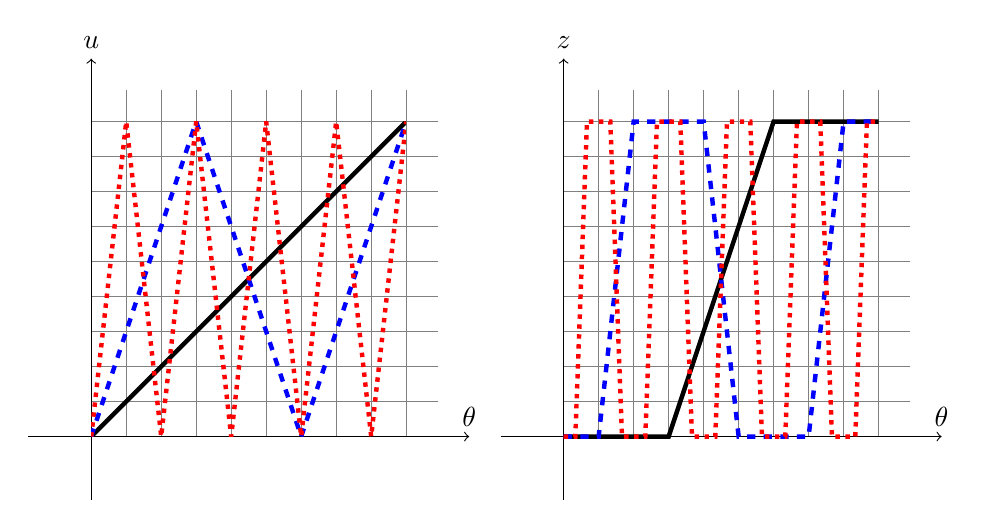
\begin{tikzpicture}[
xscale=4,
yscale=4,
point/.style={circle,inner sep=0,minimum size=1mm,fill=black},
nodepadding/.style={circle,inner sep=0,minimum size=6mm},
unselected/.style={draw=black, densely dashed},
selected/.style={draw=black},
first/.style={ultra thick},
second/.style={ultra thick,blue,dashed},
third/.style={ultra thick,red,dotted},
]

\begin{scope}[shift={(0,0)}]
\foreach \i in {1,...,9} {
    \draw [very thin,gray] (\i/9,-0.0) -- (\i/9,1.1);
    \draw [very thin,gray] (-0.0,\i/9) -- (1.1,\i/9);
}
   
\draw[->] (-0.2,0) -- (1.2,0) node[above] {$\LexUVar$};
\draw[->] (0,-0.2) -- (0,1.2) node[above] {$\LexLVarU$};

\begin{scope}
\clip(0,0) rectangle (1,1);
\draw [first] (0,0) -- (1,1);
\draw [second] (0,0) -- (1/3,1) -- (2/3, 0) -- (1,1);
\draw [third] (0,0) -- (1/9,1) -- (2/9,0) -- (3/9,1) -- (4/9,0) -- (5/9,1) -- (6/9,0) -- (7/9,1) -- (8/9, 0) -- (9/9,1);
% \draw [thick,dotted] 
% (0/27,0) -- (1/27,1) -- (2/27, 0) -- (3/27,1) -- (4/27,0) -- (5/27,1) -- (6/27, 0) -- (7/27,1) -- (8/27, 0) -- (9/27,1) --
% (10/27,0) -- (11/27,1) -- (12/27, 0) -- (13/27,1) -- (14/27,0) -- (15/27,1) -- (16/27, 0) -- (17/27,1) -- (18/27, 0) -- (19/27,1) --
% (20/27,0) -- (21/27,1) -- (22/27, 0) -- (23/27,1) -- (24/27,0) -- (25/27,1) -- (26/27, 0) -- (27/27,1);
\end{scope}

\end{scope}

\begin{scope}[shift={(1.5,0)}]
\foreach \i in {1,...,9} {
    \draw [very thin,gray] (\i/9,-0.0) -- (\i/9,1.1);
    \draw [very thin,gray] (-0.0,\i/9) -- (1.1,\i/9);
}
   
\draw[->] (-0.2,0) -- (1.2,0) node[above] {$\LexUVar$};
\draw[->] (0,-0.2) -- (0,1.2) node[above] {$\ReformZ$};

\begin{scope}
% \clip(0,0) rectangle (1,1);
\draw [first] (0,0) -- (1/3,0) -- (2/3, 1) -- (1,1);
\draw [second] (0,0) -- (1/9,0) -- (2/9, 1) -- (3/9,1) -- (4/9,1) -- (5/9,0) -- (6/9, 0) -- (7/9,0) -- (8/9, 1) -- (9/9,1);
\draw [third]
(0/27,0) -- (1/27,0) -- (2/27, 1) -- (3/27,1) -- (4/27,1) -- (5/27,0) -- (6/27, 0) -- (7/27,0) -- (8/27, 1) -- (9/27,1) --
(10/27,1) -- (11/27,0) -- (12/27, 0) -- (13/27,0) -- (14/27,1) -- (15/27,1) -- (16/27, 1) -- (17/27,0) -- (18/27, 0) -- (19/27,0) --
(20/27,1) -- (21/27,1) -- (22/27, 1) -- (23/27,0) -- (24/27,0) -- (25/27,0) -- (26/27, 1) -- (27/27,1)
;
\end{scope}

\end{scope}

\end{tikzpicture}
\caption{Plot of $\LexLVarU$ and $\ReformZ$ in $\OptSolSet(\text{\hyperref[eq:SATBilevelLexProgrammingLowerLevel]{P${}_{\text{lex}}^{\text{low}}(3, \LexUVar)$}})$.  
The solid black lines represent $\LexLVarU_3$ and $\ReformZ_3$, the dashed blue lines represent $\LexLVarU_2$ and $\ReformZ_2$, and the dotted red lines represent $\LexLVarU_1$ and $\ReformZ_1$.
}
\label{fig:plot}
\end{figure}

\begin{lemma}
\label{lemma:PenToLex}
It holds that $\OptValFunc\eqref{eq:SATBLPMultVariables} = \OptValFunc\eqref{eq:SATBilevelLexProgramming}$.
\end{lemma}

\begin{proof}
We first show that $\OptValFunc\eqref{eq:SATBLPMultVariables} \ge \OptValFunc\eqref{eq:SATBilevelLexProgramming}$.
Suppose $\SATBooleanFormula$ is satisfiable, and let $\BinaryVector$ be a binary vector satisfying $\SATBooleanFormula$, $\LexUVar = (2/3) (1 + \sum_{i = 1}^{\NVariables} \BinaryVector_i/3^{\NVariables + 1 - i})$ and $(\ReformZ, \ReformAugFrac, \LexLVarS, \LexLVarT, \LexLVarU) \in \OptSolSet\eqref{eq:SATBilevelLexProgrammingLowerLevel}$.
By Lemma~\ref{lemma:LexLowerLevelSolution}~\ref{lemma:LexLowerLevelSolutionAssertionThree}, we have $\ReformZ_i = \BinaryVector_i$ for $i = 1, \ldots, \NVariables$, $\ReformZ_{\NVariables + 1} = 1$, $\ReformAugFrac_i = |\ReformZ_i - 1/2| = 1/2$ for $i = 1, \ldots, \NVariables + 1$.
Therefore, $B_{\SATBooleanFormula} \ReformZ \ge b_{\SATBooleanFormula}$, and $(\LexUVar, \ReformZ, \ReformAugFrac, \LexLVarS, \LexLVarT, \LexLVarU)$ is feasible for~\eqref{eq:SATBilevelLexProgramming} and
$$
\OptValFunc\eqref{eq:SATBilevelLexProgramming}
\le
2 \sum_{i = 1}^{n} \left(\ReformZ_{\NVariables + 1} - 2 \ReformAugFrac_i \right) - \frac{2}{n} \sum_{i = 1}^n \ReformAugFrac_i
=
-1
=
\OptValFunc\eqref{eq:SATBLPMultVariables}.
$$
If $\SATBooleanFormula$ is unsatisfiable, we can show
$
\OptValFunc\eqref{eq:SATBilevelLexProgramming}
\le
0
=
\OptValFunc\eqref{eq:SATBLPMultVariables}
$
with $\LexUVar = 1/6$.

Next, we show that $\OptValFunc\eqref{eq:SATBLPMultVariables} \le \OptValFunc\eqref{eq:SATBilevelLexProgramming}$.
To this end, we prove that the objective value of any feasible solution to \eqref{eq:SATBilevelLexProgramming} is larger than or equal to $\OptValFunc\eqref{eq:SATBLPMultVariables}$.
Let $(\LexUVar, \ReformZ, \ReformAugFrac, \LexLVarS, \LexLVarT, \LexLVarU)$ be any feasible solution to \eqref{eq:SATBilevelLexProgramming}.
Then, we have $0 \le \ReformZ_i \le 1$, $\ReformAugFrac_i = |\ReformZ_i - 1/2|$ for $i = 1, \ldots, \NVariables + 1$, and $B_{\SATBooleanFormula} \ReformZ \ge b_{\SATBooleanFormula}$.
Therefore, $(\ReformZ, \ReformAugFrac)$ is feasible for \eqref{eq:SATBLPMultVariables}, and hence
$$
2 \sum_{i = 1}^{n} \left(\ReformZ_{\NVariables + 1} - 2 \ReformAugFrac_i \right) - \frac{2}{n} \sum_{i = 1}^n \ReformAugFrac_i
\ge \OptValFunc\eqref{eq:SATBLPMultVariables}.
$$
Since $(\LexUVar, \ReformZ, \ReformAugFrac, \LexLVarS, \LexLVarT, \LexLVarU)$ was an arbitrary feasible solution to \eqref{eq:SATBilevelLexProgramming}, it follows that $\OptValFunc\eqref{eq:SATBLPMultVariables} \le \OptValFunc\eqref{eq:SATBilevelLexProgramming}$.
\MyQED
\end{proof}

Next, we aim to reformulate the lexicographic LP~\eqref{eq:SATBilevelLexProgrammingLowerLevel} as a single-objective LP.  
There is a substantial body of literature on transforming lexicographic LPs into LPs.  
For example, Sherali~\cite{sherali1982equivalent} and Sherali and Soyster~\cite{sherali1983preemptive} explored approaches based on weighted sums of the objectives.  
However, these techniques are difficult to apply to~\eqref{eq:SATBilevelLexProgrammingLowerLevel}: Since the number of objectives increases with $\NVariables$, it is nontrivial to design appropriate weights of polynomial size to combine the objectives.
Nevertheless, since~\eqref{eq:SATBilevelLexProgrammingLowerLevel} has a special structure, we can derive an equivalent LP of polynomial size using a tailored argument.
Consider
\begin{align}
\min_{\LexUVar, \ReformZ, \ReformAugFrac, \LexLVarS, \LexLVarT, \LexLVarU} \ & 
2 \sum_{i = 1}^{n} \left(\ReformZ_{\NVariables + 1} - 2 \ReformAugFrac_i \right) - \frac{2}{n} \sum_{i = 1}^n \ReformAugFrac_i
\tag{P${}_{\text{weight}}^{\text{}}(\SATBooleanFormula)$}
\label{eq:SATBilevelWeightedProblem}
\\
\text{s.t.} \ &
B_{\SATBooleanFormula} \ReformZ \ge b_{\SATBooleanFormula}, 
0 \le \LexUVar \le 1, \notag \\
&
(\ReformZ, \ReformAugFrac, \LexLVarS, \LexLVarT, \LexLVarU) 
\in
\OptSolSet\eqref{eq:SATBilevelWeightedProblemLowerLevel},
\notag 
\end{align}
where
\begin{align}
\min_{\ReformZ, \ReformAugFrac, \LexLVarS, \LexLVarT, \LexLVarU} \ & 
\sum_{i = 1}^{\NVariables + 1}
\LexWeightValue^i (\LexLVarS_i + \LexLVarT_i)
+ 
\sum_{i = 1}^{\NVariables + 1} \frac{1}{4^{\NVariables - i + 1}} \ReformAugFrac_i
\tag{P${}_{\text{weight}}^{\text{low}}(\NVariables + 1, \LexUVar)$}
\label{eq:SATBilevelWeightedProblemLowerLevel}
\\
\text{s.t.} \
&
(\ReformZ, \ReformAugFrac, \LexLVarS, \LexLVarT, \LexLVarU)
\in
\FeasSolSet\eqref{eq:SATBilevelLexProgrammingLowerLevel}.
\notag 
\end{align}
We show that $\OptValFunc\eqref{eq:SATBilevelLexProgramming} = \OptValFunc\eqref{eq:SATBilevelWeightedProblem}$.
\begin{lemma}
\label{lemma:LexToWeighted}
\mbox{}
\begin{enumerate}
\item
\label{lemma:LexToWeightedAssertionOne}
For any $\NVariables \ge 1$ and $\LexUVar \in [0, 1]$, $\OptSolSet\eqref{eq:SATBilevelLexProgrammingLowerLevel} = \OptSolSet\eqref{eq:SATBilevelWeightedProblemLowerLevel}$.
\item
It holds that $\OptValFunc\eqref{eq:SATBilevelLexProgramming} = \OptValFunc\eqref{eq:SATBilevelWeightedProblem}$.
\end{enumerate}
\end{lemma}

See \IPCO{the full version of the paper~\cite{sugishita2025complexitybilevellinearprogramming}}{Appendix~\ref{sec:proof_of_lemma_lex_to_weighted}} for the proof.
As the last step, we remove $B_{\SATBooleanFormula} \ReformZ \ge b_{\SATBooleanFormula}$ from the upper-level problem using Lemma~\ref{lemma:PenaltyReformulation} and obtain
\begin{align}
\min_{\LexUVar, \ReformZ, \ReformAugFrac, \LexLVarS, \LexLVarT, \LexLVarU, \ReformPen} \ & 
2 \sum_{i = 1}^{n} \left(\ReformZ_{\NVariables + 1} - 2 \ReformAugFrac_i \right) - \frac{2}{n} \sum_{i = 1}^n \ReformAugFrac_i + M \ReformPen
\tag{P${}_{\text{}}^{\text{}}(\SATBooleanFormula)$}
\label{eq:SATBLPLast}
\\
\text{s.t.} \
&
(\ReformZ, \ReformAugFrac, \LexLVarS, \LexLVarT, \LexLVarU, \ReformPen) 
\in
\OptSolSet\eqref{eq:SATBLPLastLowerLevel},
\notag 
\end{align}
where
\begin{align}
\min_{\ReformZ, \ReformAugFrac, \LexLVarS, \LexLVarT, \LexLVarU, \ReformPen} \ & 
\sum_{i = 1}^{\NVariables + 1}
\LexWeightValue^i (\LexLVarS_i + \LexLVarT_i)
+ 
\sum_{i = 1}^{\NVariables + 1} \frac{1}{4^{\NVariables - i + 1}} \ReformAugFrac_i
\tag{P${}_{\text{}}^{\text{low}}(\SATBooleanFormula, \LexUVar)$}
\label{eq:SATBLPLastLowerLevel}
\\
\text{s.t.} \
&
B_{\SATBooleanFormula} \ReformZ + \ReformPen \OneVector \ge b_{\SATBooleanFormula},
0 \le \LexUVar \le 1, 
0 \le \ReformPen \le 1,
\notag \\
&
(\ReformZ, \ReformAugFrac, \LexLVarS, \LexLVarT, \LexLVarU)
\in
\FeasSolSet\eqref{eq:SATBilevelLexProgrammingLowerLevel},
\notag 
\end{align}
% Penalty coefficient
with $M = 3 (5 \NVariables + 7) 4^{\SolutionSizeEstimate(5 \NVariables + 3, \Size{6}) +1}$.
\phantomsection\label{Rev:WhyECanBeBounded} We note that the penalty term $e$ can be bounded from above (see Lemma~\ref{lemma:PenaltyReformulation}).

\begin{lemma}
\label{lemma:WeightedToPenalty}
It holds that $\OptValFunc\eqref{eq:SATBilevelWeightedProblem} = \OptValFunc\eqref{eq:SATBLPLast}$.
\end{lemma}
The proof is in \IPCO{the full version of the paper~\cite{sugishita2025complexitybilevellinearprogramming}}{Appendix~\ref{sec:ProofOfLemmaWeightedToPenalty}}.
Note that the \EncodingSize{} of \eqref{eq:SATBLPLast} is polynomial in $\NVariables$.
\begin{lemma}
\label{lemma:ValueOfTransformedInstance}
\mbox{}
\begin{enumerate}
\item
Suppose $\SATBooleanFormula$ is satisfiable.
Then, $\OptValFunc\eqref{eq:SATBLPLast} = -1$.
\item
Suppose $\SATBooleanFormula$ is unsatisfiable.
Then, $\OptValFunc\eqref{eq:SATBLPLast} = 0$.
\end{enumerate}
\end{lemma}

\begin{proof}
It follows from Lemmata~\ref{lemma:SATBLPFirst}-\ref{lemma:WeightedToPenalty}.
\MyQED
\end{proof}

Theorem~\ref{theorem:ValueOfBLPWithSingleUpperLevelVariableIsNPHard} follows immediately from the above argument.

\begin{proof}[Proof of Theorem~\ref{theorem:ValueOfBLPWithSingleUpperLevelVariableIsNPHard}]
\phantomsection\label{Rev:LogSpaceReduction}
The inclusion in \ClassNP{} follows from~\cite{Buchheim2023}.
% the fact that the decision version of general bilevel LP is in \ClassNP{} \cite{Buchheim2023}.
By Lemma~\ref{lemma:ValueOfTransformedInstance}, the above transformation gives a logarithmic-space reduction \cite{papadimitriou1993computational} from \ThreeSAT{} to \ValueOfBLPWithSingleUpperLevelVariable{}.
Since \ThreeSAT{} is \ClassNP{}-complete, \ValueOfBLPWithSingleUpperLevelVariable{} is \ClassNP{}-hard.
\MyQED
\end{proof}

A few remarks are in order.
First, \phantomsection\label{Rev:Approximation} by adding 1 (or, equivalently, by adding a variable fixed to 1) to the objective of~\eqref{eq:SATBLPLast}, one can obtain an instance whose optimal objective value is $0$ if $\SATBooleanFormula$ is satisfiable and $1$ otherwise.
Thus, even approximate versions of \ValueOfBLPWithSingleUpperLevelVariable{} are $\ClassNP$-hard (See Corollary 4.6 in Jeroslow~\cite{Jeroslow1985}).
Second, instance~\eqref{eq:SATBLPLast} contains constants of exponential magnitude.  
% As a result, there is a possibility that a bilevel LP with a single variable and no upper-level constraints is not strongly \ClassNP{}-hard.  
Consequently, a bilevel LP with a single variable and no upper-level constraints may not be strongly \ClassNP{}-hard.
In particular, such instances may admit pseudo-polynomial algorithms.
\phantomsection\label{Rev:Pessimistic} Third, our proof of \ClassNP{}-hardness for the decision version of the optimistic formulation of bilevel LP also carries over to the pessimistic formulation. Recall that in the pessimistic formulation the follower, when faced with multiple optimal solutions, selects the one least favorable to the leader. Since the lower-level problem in our construction has a unique optimal solution, the optimal objective value of the pessimistic variant of \eqref{eq:SATBLPLast} coincides with that of the optimistic variant.
Fourth, the argument of Basu \EtAl{}~\cite{BasuEtAl2021} shows that the feasible set of a bilevel LP is the union of at most exponentially many polyhedra.
We observe that instance~\eqref{eq:SATBLPLast}, a bilevel LP with a single upper-level variable and no upper-level constraints, requires exponentially many polyhedra to describe its feasible set.
Formally, we have the following result, proven in \IPCO{the full version of the paper~\cite{sugishita2025complexitybilevellinearprogramming}}{Appendix~\ref{sec:ProofOfPropNumberOfPolyhedra}}.
\begin{proposition}
\label{prop:NumberOfPolyhedra}
Let $q$ be the smallest integer such that there exists polyhedra $Q_1, \ldots, Q_q$ satisfying $\FeasSolSet\eqref{eq:SATBLPLast} = \cup_{j = 1 \ldots, q} Q_j$.
Then, $q \ge 2^{n}$.
In other words, any representation of $\FeasSolSet\eqref{eq:SATBLPLast}$ as a union of polyhedra requires exponentially many polyhedra in $n$.
\end{proposition}

\section{Reformulation of Combinatorial Optimization Problem}
\label{sec:ImplicationOfTheorem}

In this section, we briefly present a reformulation of combinatorial optimization problems into instances of \BLPWithSingleUpperLevelVariable{}.
\phantomsection\label{Rev:MotivationOfReformulationOfCombProblem} Given a \ClassNP{}-hard combinatorial optimization problem, one can construct a reduction from its decision version to the decision version of \BLPWithSingleUpperLevelVariable{}.
However, by exploiting the techniques developed in Section~\ref{sec:ProofOfTheorem1}, one can in fact design a transformation that preserves optimal solutions, in the sense that an optimal solution to the original combinatorial problem can be constructed from one for the resulting \BLPWithSingleUpperLevelVariable{} instance, and vice versa.
Consider the following 0-1 integer LP:
\begin{align}
\min_{\ReformZ} \{ c^{\top} \ReformZ 
:
A \ReformZ \ge a, \ReformZ \in \{0, 1\}^\IPNVariables\},
\tag{C}
\label{eq:Knapsack}
\end{align}
where $c \in \mathbb{Q}^{\IPNVariables}$, $A \in \mathbb{Q}^{\NConstraints \times \IPNVariables}$, and $a \in \mathbb{Q}^{\NConstraints}$.  
We assume that \eqref{eq:Knapsack} has at least one feasible solution, which holds when it is a 0-1 integer LP formulation of the knapsack or traveling salesman problem over a fully-connected graph.
By appropriate scaling if necessary, we may assume $a_j \in [-1,1]$ for all $j = 1, \ldots, \NConstraints$.  
We first replace the binary variables using the lexicographic LP~(\hyperref[eq:SATBilevelLexProgrammingLowerLevel]{P${}_{\text{lex}}^{\text{low}}(\IPNVariables, \LexUVar)$}) or its LP equivalent~(\hyperref[eq:SATBilevelWeightedProblemLowerLevel]{P${}_{\text{weight}}^{\text{low}}(\IPNVariables, \LexUVar)$}) (Lemma~\ref{lemma:LexToWeighted}~\ref{lemma:LexToWeightedAssertionOne} is stated for $\IPNVariables \ge 2$ but it is straightforward to show that it also holds for $\IPNVariables = 1$):
\begin{align}
\min_{\LexUVar, \ReformZ, \ReformAugFrac, \LexLVarS, \LexLVarT, \LexLVarU} \ & c^{\top} \ReformZ 
\tag{C$_{\text{mult}}$}
\label{eq:KnapsackMiddle}
\\
\text{s.t.} \ 
&
A \ReformZ \ge a, 0 \le \LexUVar \le 1, \ReformAugFrac_{i} \ge 1/2, \ \forall i = 1, \ldots, n,
\label{eq:KnapsackBLPWithUpperLevelConstraintConstraint}
\\
&
(\ReformZ, \ReformAugFrac, \LexLVarS, \LexLVarT, \LexLVarU) \in 
\OptSolSet(\text{\hyperref[eq:SATBilevelWeightedProblemLowerLevel]{P${}_{\text{weight}}^{\text{low}}(\IPNVariables, \LexUVar)$}}),
\notag
\end{align}
where $\LexUVar \in \mathbb{R}$, and $\ReformZ, \ReformAugFrac, \LexLVarS, \LexLVarT, \LexLVarU \in \mathbb{R}^{\IPNVariables}$.  
For each $i = 1, \ldots, \IPNVariables$, the optimality of the lower-level problem implies $\ReformAugFrac_i = |\ReformZ_i - 1/2|$, thus the condition $\ReformAugFrac_i \geq 1/2$ enforces $\LexUVar$ to be such that $\ReformZ_i \in \{0,1\}$.  
Next, we replace the constraints~\eqref{eq:KnapsackBLPWithUpperLevelConstraintConstraint} with a penalty term added to the objective:
\begin{align}
\min_{\LexUVar, \ReformZ, \ReformAugFrac, \LexLVarS, \LexLVarT, \LexLVarU, \ReformPen}
\{
c^{\top} \ReformZ + M \ReformPen 
:
(\ReformZ, \ReformAugFrac, \LexLVarS, \LexLVarT, \LexLVarU, \ReformPen) \in 
\OptSolSet\eqref{eq:KnapsackLastLowerLevel}
\},
\tag{C$_{\mathrm{single}}$}
\label{eq:KnapsackLast}
\end{align}
where
\begin{align}
\min_{\ReformZ, \ReformAugFrac, \LexLVarS, \LexLVarT, \LexLVarU, \ReformPen} \ & 
\sum_{i = 1}^{\IPNVariables}
\LexWeightValue^i (\LexLVarS_i + \LexLVarT_i)
+ 
\sum_{i = 1}^{\IPNVariables} \frac{1}{4^{\IPNVariables - i}} \ReformAugFrac_i
\tag{C${}_{\text{single}}^{\text{low}}(\LexUVar)$}
\label{eq:KnapsackLastLowerLevel}
\\
\text{s.t.} \
&
A \ReformZ + \ReformPen \OneVector \ge a, \ReformAugFrac_{i} + \ReformPen \ge 1/2, \ \forall i = 1, \ldots, \IPNVariables, 
\notag
\\
&
0 \le \LexUVar \le 1, 
0 \le \ReformPen \le 1,
\notag \\
&
(\ReformZ, \ReformAugFrac, \LexLVarS, \LexLVarT, \LexLVarU)
\in
\FeasSolSet(\text{\hyperref[eq:SATBilevelLexProgrammingLowerLevel]{P${}_{\text{lex}}^{\text{low}}(\IPNVariables, \LexUVar)$}}).
\notag 
\end{align}
and $M$ is a penalty coefficient.  
It is straightforward to verify that both instances \eqref{eq:KnapsackMiddle} and \eqref{eq:KnapsackLast} admit optimal solutions for any value of $M$.  
For example, \eqref{eq:KnapsackLast} has a feasible solution given by $\LexUVar = 0$, $\ReformZ = \ReformAugFrac = \LexLVarS = \LexLVarT = \LexLVarU = \ZeroVector$, and $\ReformPen = 1$.  
Moreover, \eqref{eq:KnapsackLast} cannot be unbounded since all the variables are bounded, thus guaranteeing the existence of an optimal solution.  
Therefore, by invoking Lemma~\ref{lemma:PenaltyReformulation}, one can compute a penalty coefficient $M$ of polynomial size (in the size of~\eqref{eq:Knapsack}) such that $\OptValFunc\eqref{eq:Knapsack} = \OptValFunc\eqref{eq:KnapsackLast}$.
In fact, it is straightforward to see the following: 
$\OptSolSet\eqref{eq:KnapsackLast} = \{ (\LexUVar, \ReformZ, \ReformAugFrac, \LexLVarS, \LexLVarT, \LexLVarU, \ReformPen) \in \FeasSolSet\eqref{eq:KnapsackLast} : \ReformZ\in \OptSolSet\eqref{eq:Knapsack} \}$.

\section{Complexity of Local Search}
\label{sec:ComplexityOfVerifyingASolution}

To further understand the computational complexity of \BLPWithSingleUpperLevelVariable{}, in the remainder of the paper, we study the complexity of searching for a solution.
We begin by discussing the \ClassCoNP{}-completeness of deciding whether a given point is a globally optimal solution.
We then turn our attention to the problem of finding a locally optimal solution.
We show that it is possible to compute a locally optimal solution in polynomial time.

Consider the following decision problem:
\begin{align*}
&
\parbox{0.75\textwidth}{Given a rational instance \eqref{eq:NotationBLP} and a rational point $(x_1, x_2)$, is it an optimal solution?}
\label{GlobalOptimalProblemAnchor}
\tag{\GlobalOptimalProblemName{}}
\end{align*}

Using instance~\eqref{eq:SATBLPLast}, we obtain the following result, which is proven in \IPCO{the full version of the paper~\cite{sugishita2025complexitybilevellinearprogramming}}{Appendix~\ref{sec:ProofOfTheoremComplexityOfVerifyingOptimalSolution}}.
\begin{proposition}
\label{theorem:ComplexityOfVerifyingOptimalSolution}
The decision problem \GlobalOptimalProblem{} is \ClassCoNP{}-complete.
\end{proposition}

Proposition~\ref{theorem:ComplexityOfVerifyingOptimalSolution} shows that merely deciding whether a given point is an optimal solution is \ClassCoNP{}-complete.
Therefore, searching for a globally optimal solution is likely to be computationally intractable.
A natural question is whether replacing global optimality with local optimality leads to a tractable problem.

We say that $(\bar{x}_1, \bar{x}_2) \in \mathbb{R}^{\NVariables + 1}$ is a \emph{locally optimal solution} to \eqref{eq:NotationBLP} if $(\bar{x}_1, \bar{x}_2) \in \FeasSolSet\eqref{eq:NotationBLP}$ and there exists $\epsilon > 0$ such that
$$
c_{2 1}^{\top} \bar{x}_1 + c_{2 2} \bar{x}_2 \le c_{2 1}^{\top} x_1 + c_{2 2} x_2,
\quad \forall\, (x_1, x_2) \in \FeasSolSet\eqref{eq:NotationBLP} \cap \mathcal{B}_{\epsilon}(\bar{x}_1, \bar{x}_2),
$$
where
$
\mathcal{B}_{\epsilon}(\bar{x}_1, \bar{x}_2) = \{ (x_1, x_2) : \| (x_1, x_2) - (\bar{x}_1, \bar{x}_2) \|_{\infty} \le \epsilon \}.
$
The following result holds.
\begin{theorem}
\label{theorem:ComplexityOfLocalSearch}
There exists a polynomial-time algorithm that finds a locally optimal solution to a rational instance of~\eqref{eq:NotationBLP}.
\end{theorem}

See \IPCO{the full version of the paper~\cite{sugishita2025complexitybilevellinearprogramming}}{Appendix~\ref{sec:ProofOfTheoremComplexityOfLocalSearch}} for the proof.
We show that if there is a local optimal solution, there is a rational one of polynomial size.
Thus, we apply a binary search on the upper-level variable $x_2$ to find a local optimal solution.
This result contrasts with a well-known result by Vicente \EtAl{}~\cite{vicente1994descent}, which shows that recognizing local optimality is \ClassNP{}-hard in the general case.
% Similarly, \cite{ProkopyevRalphs2024} showed that search for a local optimal solution is \ClassNP{}-hard.
Thus, Theorem~\ref{theorem:ComplexityOfLocalSearch} suggests a fundamental difference between general bilevel LPs and \BLPWithSingleUpperLevelVariable{}.

\begin{credits}
\subsubsection{\ackname} 
This study was funded by the FRQ-IVADO Research Chair in Data Science for Combinatorial Game Theory.

\subsubsection{\discintname}
The authors have no competing interests to declare that are
relevant to the content of this article.
\end{credits}
%
% ---- Bibliography ----
%
% BibTeX users should specify bibliography style 'splncs04'.
% References will then be sorted and formatted in the correct style.
%
\bibliographystyle{splncs04}
\bibliography{references}

\ifIPCOFlag
\else
\clearpage

\begin{appendix}

\section{Proof of Lemma~\ref{lemma:SolutionSizeEstimate}}
\label{sec:proof_of_lemma_solution_size_estimate}

% To prove Lemma~\ref{lemma:SolutionSizeEstimate}, we use the following result.
% \begin{lemma}
% \label{lemma:estimate-of-primal-linear-inequality}
% Let $A \in \mathbb{Q}^{\NConstraints \times \NVariables}$, $b \in \mathbb{Q}^{\NConstraints}$, $c \in \mathbb{Q}^{\NVariables}$, and $\sigma$ be the maximum \EncodingSize{} of the entries in $A$ and $b$.
% % p134
% % where each inequality in Ax 5b has size at most p.
% % P44
% % each row of the matrix [A b] has size at most p
% % \begin{enumerate}
% % \item
% % If $Q$ is nonempty, then $Q$ contains a rational point of size polynomially bounded by $\sigma$ and $n$.
% % \item 
% % All the vertices and extreme rays of $Q$ are rational of \EncodingSize{} polynomially bounded by $\sigma$ and $n$.
% % \item 
% If $\min_{x \in \mathbb{R}^{\NVariables}} \{ c^{\top} x : A x \ConstraintSense b\}$ has an optimal solution, it has a rational optimal solution whose \EncodingSize{} is less than or equal to $4\NVariables^2(\NVariables+1)(\sigma+1)$.
% % \end{enumerate}
% \end{lemma}

\begin{proof}
The feasible set of $\eqref{eq:SolutionSizeEstimateBLP}$ is the union of polyhedra~\cite{BasuEtAl2021}.
Indeed,
\begin{align*}
\FeasSolSet\eqref{eq:SolutionSizeEstimateBLP}
&=
\left\{
\begin{pmatrix}
x_1 \\ x_2
\end{pmatrix}
:
\exists \lambda \text{ s.t. }
\begin{array}{l}
A_{2 1} x_1 + A_{2 2} x_2 \ge b_2, \\
A_{1 1} x_1 + A_{1 2} x_2 \ge b_1, \\
\lambda^{\top} ( A_{1 1} x_1 + A_{1 2} x_2 - b_1) = 0, \\
A_{1 1}^{\top} \lambda = c_{1 1}, \\
\lambda \ge 0
\end{array}
\right\}
\\
&=
\bigcup_{\omega \in \{0, 1\}^{\NConstraints_1}}
\left\{
\begin{pmatrix}
x_1 \\ x_2
\end{pmatrix}
:
\exists \lambda \text{ s.t. }
\begin{array}{l}
A_{2 1} x_1 + A_{2 2} x_2 \ge b_2, \\
A_{1 1} x_1 + A_{1 2} x_2 \ge b_1, \\
\omega^{\top} ( A_{1 1} x_1 + A_{1 2} x_2 - b_1) = 0, \\
(1 - \omega)^{\top} \lambda = 0, \\
A_{1 1}^{\top} \lambda = c_{1 1}, \\
\lambda \ge 0
\end{array}
\right\}.
\end{align*}
That is, $\FeasSolSet\eqref{eq:SolutionSizeEstimateBLP} = \cup_{\omega \in \Omega} U_{\omega}$, where
$$
\Omega = \{
\omega \in \{0, 1\}^{\NConstraints_1} : \exists \lambda \text{ s.t. } 
(1 - \omega)^{\top} \lambda = 0, 
A_{1 1}^{\top} \lambda = c_{1 1}, 
\lambda \ge 0
\}
$$
and for each $\omega \in \Omega$,
\begin{align*}
% \FeasSolSet\eqref{eq:SolutionSizeEstimateBLP}
% =
% \bigcup_{\omega \in \Omega}
U_{\omega} =
\left\{
\begin{pmatrix}
x_1 \\ x_2
\end{pmatrix}
:
\begin{array}{l}
A_{2 1} x_1 + A_{2 2} x_2 \ge b_2, \\
A_{1 1} x_1 + A_{1 2} x_2 \ge b_1, \\
\omega^{\top} ( A_{1 1} x_1 + A_{1 2} x_2 - b_1) = 0 \\
% (1 - \omega)^{\top} \lambda = 0, \\
% A_{1 1}^{\top} \lambda = c_{1 1}, \\
% \lambda \ge 0.
\end{array}
\right\}.
\end{align*}
Let 
\begin{align}
\min_{x_1, x_2} \{c_{2 1}^{\top} x_1 + c_{2 2}^{\top} x_2 : (x_1, x_2) \in U_{\omega} \}
\label{eq:DecomposedLP}
\tag{$\mathrm{P}_{\mathrm{decomp}}(\omega)$}
\end{align}
and observe that $\OptValFunc\eqref{eq:SolutionSizeEstimateBLP} = \min_{\omega \in \Omega} \OptValFunc\eqref{eq:DecomposedLP}$ and $\OptSolSet\eqref{eq:SolutionSizeEstimateBLP} = \cup_{\omega \in \Omega'} \OptSolSet(\mathrm{P}_{\mathrm{decomp}}(\omega))$, where $\Omega' = \Argmin_{\omega \in \Omega} \OptValFunc\eqref{eq:DecomposedLP}$.
Note that each $U_\omega$ can be defined by inequalities with coefficients of size at most $\sigma$.
Thus, by Lemma~\ref{lemma:estimate-of-primal-linear-inequality}, for each $\omega \in \Omega$, $\OptSolSet\eqref{eq:DecomposedLP}$ contains a rational point of size $\SolutionSizeEstimate(\NVariables, \sigma)$ given it is nonempty.
\MyQED
\end{proof}

\section{Proof of Lemma~\ref{lemma:PenaltyReformulation}}
\label{sec:ProofOfLemmaPenaltyReformulation}

\begin{lemma}
\label{lemma:ZeroViolation}
Under the assumptions of Lemma~\ref{lemma:PenaltyReformulation}, for any $(x_1, x_2, e) \in \OptSolSet\eqref{eq:PenaltyAfter}$, it holds that $e = 0$.
\end{lemma}

\begin{proof}
For any $x_1 \in \mathbb{R}^{\NVariables_1}$ and $x_2 \in \mathbb{R}^{\NVariables_2}$, $(x_1, x_2) \in \FeasSolSet\eqref{eq:PenaltyBefore}$ implies $(x_1, x_2, 0) \in \FeasSolSet\eqref{eq:PenaltyAfter}$.
Thus, we have 
\begin{equation}
\OptValFunc\eqref{eq:PenaltyBefore} \ge \OptValFunc\eqref{eq:PenaltyAfter}.
\label{eq:ProofPenaltyReformulationRelaxation}
\end{equation}
For the sake of contradiction, assume that there exists $(\bar{x}_1, \bar{x}_2, \bar{\ReformPen}) \in \OptSolSet\eqref{eq:PenaltyAfter}$ such that $\bar{\ReformPen} > 0$.
Under this assumption, we show that $\OptValFunc\eqref{eq:PenaltyBefore} < \OptValFunc\eqref{eq:PenaltyAfter}$, which contradicts \eqref{eq:ProofPenaltyReformulationRelaxation}.
Let $\NConstraints'$ be the number of constraints in the lower-level problem of~\eqref{eq:PenaltyAfter}.
Following the argument in the proof of Lemma~\ref{lemma:SolutionSizeEstimate}, we can write the feasible set of \eqref{eq:PenaltyAfter} as the union of polyhedra:
$$
\FeasSolSet\eqref{eq:PenaltyAfter} = \bigcup_{\omega \in \Omega'} U_{\omega}',
$$
where $\Omega' \subset \{0, 1\}^{\NConstraints'}$ and for each $\omega \in \Omega'$, $U_{\omega}' \subset \mathbb{R}^{\NVariables + 1}$ is a rational polyhedron defined by inequalities whose coefficients are of \EncodingSize{} at most $\sigma$.
Furthermore, there is $\bar{\omega} \in \Omega'$ such that $(\bar{x}_1, \bar{x}_2, \bar{\ReformPen}) \in U_{\bar{\omega}}'$.
Now, consider the LP
\begin{equation}
\min_{x_1, x_2, \ReformPen} \{ c_{2 1}^{\top} x_1 + c_{2 2}^{\top} x_2 + M \ReformPen : (x_1, x_2, \ReformPen) \in U_{\bar{\omega}}', \ReformPen > 0 \}.
\label{eq:PenaltyAfterStrictlyPositiveLP}
\end{equation}
Since $(\bar{x}_1, \bar{x}_2, \bar{\ReformPen})$ is also an optimal solution to $\eqref{eq:PenaltyAfterStrictlyPositiveLP}$, we have $\emptyset \not= \OptSolSet\eqref{eq:PenaltyAfterStrictlyPositiveLP} \subset U_{\bar{\omega}}' \subset \OptSolSet\eqref{eq:PenaltyAfter}$.
By Lemma~\ref{lemma:estimate-of-primal-linear-inequality}, there exists a rational solution $(\tilde{x}_1, \tilde{x}_2, \tilde{\ReformPen}) \in \OptSolSet\eqref{eq:PenaltyAfterStrictlyPositiveLP}$ such that $\SizeThree{\tilde{x}_1}{\tilde{x}_2}{\tilde{\ReformPen}} \le \SolutionSizeEstimate(\NVariables + 1, \sigma)$.
In particular, we have $\tilde{\ReformPen} > 0$, implying $\tilde{\ReformPen} \ge 1 / 2^{\SolutionSizeEstimate(\NVariables + 1, \sigma)}$.
Let $(\hat{x}_1, \hat{x}_2) \in \mathbb{Q}^{\NVariables}$ be a rational optimal solution to \eqref{eq:PenaltyBefore} such that $\SizeTwo{\hat{x}_1}{\hat{x}_2} \le \SolutionSizeEstimate(\NVariables + 1, \sigma)$.
Then,
\begin{align}
&
\OptValFunc\eqref{eq:PenaltyAfter}
-
\OptValFunc\eqref{eq:PenaltyBefore}
\notag
% \label{eq:LemmaPenatyReformulationContradiction}
\\
&
\qquad
=
(c_{2 1}^{\top} \tilde{x}_1 + c_{2 2}^{\top} \tilde{x}_2 + M \tilde{\ReformPen})
-(c_{2 1}^{\top} \hat{x}_1 + c_{2 2}^{\top} \hat{x}_2)
\notag
\\
% -------------------------------------------------
&
\qquad
\ge
M \tilde{\ReformPen} 
- \|c_{2 1} \|_\infty \| \tilde{x}_1 \|_1
- \|c_{2 2} \|_\infty \| \tilde{x}_2 \|_1
- \|c_{2 1} \|_\infty \| \hat{x}_1 \|_1
- \|c_{2 2} \|_\infty \| \hat{x}_2 \|_1
\notag
\\
% -------------------------------------------------
&
\qquad
\ge
M \tilde{\ReformPen} 
- c_\infty \NVariables_1 \| \tilde{x}_1 \|_\infty
- c_\infty \NVariables_2 \| \tilde{x}_2 \|_\infty
- c_\infty \NVariables_1 \| \hat{x}_1 \|_\infty
- c_\infty \NVariables_2 \| \hat{x}_2 \|_\infty
\notag
\\
% -------------------------------------------------
&
\qquad
\ge
M/2^{\SolutionSizeEstimate(\NVariables + 1, \sigma)}
- c_{\infty} \NVariables_1 2^{\SolutionSizeEstimate(\NVariables + 1, \sigma)}
- c_{\infty} \NVariables_2 2^{\SolutionSizeEstimate(\NVariables + 1, \sigma)}
\notag
\\
& 
\qquad
\qquad
\qquad
\qquad
\qquad
\qquad
-  c_{\infty} \NVariables_1 2^{\SolutionSizeEstimate(\NVariables + 1, \sigma)}
- c_{\infty} \NVariables_2 2^{\SolutionSizeEstimate(\NVariables + 1, \sigma)}
\notag
\\
% -------------------------------------------------
&
\qquad
\ge
M/2^{\SolutionSizeEstimate(\NVariables + 1, \sigma)}
- 2 c_{\infty} \NVariables 2^{\SolutionSizeEstimate(\NVariables + 1, \sigma)}
\notag
\\
% -------------------------------------------------
&
\qquad
\ge
M/2^{\SolutionSizeEstimate(\NVariables + 1, \sigma)}
- (2/3) M/2^{\SolutionSizeEstimate(\NVariables + 1, \sigma)}
\notag
\\
% -------------------------------------------------
&
\qquad
> 0,
\notag
\end{align}
which contradicts~\eqref{eq:ProofPenaltyReformulationRelaxation}.
Therefore, for any $(\bar{x}_1, \bar{x}_2, \bar{\ReformPen}) \in \OptSolSet\eqref{eq:PenaltyAfter}$ we have $\bar{\ReformPen} = 0$.
\MyQED
\end{proof}

\begin{proof}[Lemma~\ref{lemma:PenaltyReformulation}]
We prove relation~(ii), from which relation~(i) follows directly.
We establish the following two statements: 
\begin{enumerate}[label=(A-\arabic*)]
\item
\label{item:lemma:PenaltyReformulation:StepOne}
If $(x_1, x_2, \ReformPen) \in \OptSolSet\eqref{eq:PenaltyAfter}$, then $\ReformPen = 0$ and $(x_1, x_2) \in \OptSolSet\eqref{eq:PenaltyBefore}$;
\item 
\label{item:lemma:PenaltyReformulation:StepTwo}
If $(x_1, x_2) \in \OptSolSet\eqref{eq:PenaltyBefore}$, then $(x_1, x_2, 0) \in \OptSolSet\eqref{eq:PenaltyAfter}$.
\end{enumerate}
The desired relation follows from these two assertions.

We begin with the proof of assertion~\ref{item:lemma:PenaltyReformulation:StepOne}.
Let $(x_1, x_2, \ReformPen) \in \OptSolSet\eqref{eq:PenaltyAfter}$.
By Lemma~\ref{lemma:ZeroViolation}, $\ReformPen = 0$.
It remains to show that $(x_1, x_2)$ is optimal to \eqref{eq:PenaltyBefore}. 
We show the feasibility and optimality of $(x_1, x_2)$ in order.
Since $(x_1, x_2, 0) \in \OptSolSet\eqref{eq:PenaltyAfter}$, it follows that $(x_1, x_2)$ satisfies all the linear inequalities in~\eqref{eq:PenaltyBefore}.
Thus, $(x_1, x_2)$ is feasible for \eqref{eq:PenaltyBefore} if and only if $x_1$ is optimal to the lower-level problem of~\eqref{eq:PenaltyBefore} given $x_2$.
To derive a contradiction, suppose $x_1$ is not optimal to the lower-level problem of~\eqref{eq:PenaltyBefore}.
Then, there exists $\bar{x}_1$ feasible to the lower-level problem of~\eqref{eq:PenaltyBefore} such that $c_{1 1}^{\top} \bar{x}_1 < c_{1 1}^{\top} x_1$.
Let $V \ge 1$ be a real number such that
$$
\bar{A}_{2 1} \bar{x}_1 + \bar{A}_{2 2} x_2 + V \ge \bar{b}_2.
$$
Define
$$
\hat{x}_1 = \frac{V - 1}{V} x_1 + \frac{1}{V} \bar{x}_1, \hat{e} = 1.
$$
Then, $(\hat{x}_1, \hat{e})$ is feasible to the lower-level problem of~\eqref{eq:PenaltyAfter}, and its objective value is strictly smaller than that of $(x_1, 0)$, a contradiction to the feasibility of $(x_1, x_2, 0)$ to \eqref{eq:PenaltyAfter}.
Thus, $x_1$ is indeed optimal to the lower-level problem of~\eqref{eq:PenaltyBefore}, and $(x_1, x_2)$ is a feasible solution to~\eqref{eq:PenaltyBefore}.
The objective value of $(x_1, x_2)$ in instance~\eqref{eq:PenaltyBefore} is $c_{21}^{\top} x_1 + c_{22}^{\top} x_2$.
By assumption $(x_1, x_2, 0) \in \OptSolSet\eqref{eq:PenaltyAfter}$, we have $\OptValFunc\eqref{eq:PenaltyAfter} = c_{21}^{\top} x_1 + c_{22}^{\top} x_2$.
In light of \eqref{eq:ProofPenaltyReformulationRelaxation}, $(x_1, x_2)$ is optimal for \eqref{eq:PenaltyBefore} and $\OptValFunc\eqref{eq:PenaltyBefore} = \OptValFunc\eqref{eq:PenaltyAfter}$.

We now prove assertion~\ref{item:lemma:PenaltyReformulation:StepTwo}.
Let $(x_1, x_2) \in \OptSolSet\eqref{eq:PenaltyBefore}$.
We claim that $(x_1, 0)$ is optimal to the lower-level problem of~\eqref{eq:PenaltyAfter}.
Suppose the contrary.
Then thre exists a feasible solution $(\hat{x}_1, \hat{e})$ to the lower-level problem of~\eqref{eq:PenaltyAfter} such that $c_{1 1}^{\top} \hat{x}_1 < c_{1 1}^{\top} x_1$.
Note that $\hat{x}_1$ is feasible to the lower-level problem of~\eqref{eq:PenaltyBefore} with a strictly smaller objective value than $x_1$, a contradiction to the assumption that $(x_1, x_2) \in \FeasSolSet\eqref{eq:PenaltyBefore}$.
Therefore, $(x_1, 0)$ is optimal to the lower-level problem of~\eqref{eq:PenaltyAfter}, and we have $(x_1, x_2, 0) \in \FeasSolSet\eqref{eq:PenaltyAfter}$.
Since $\OptValFunc\eqref{eq:PenaltyBefore} = \OptValFunc\eqref{eq:PenaltyAfter}$, $(x_1, x_2, 0)$ is optimal for~\eqref{eq:PenaltyAfter}.
\MyQED
\end{proof}

\section{Proof of Lemma~\ref{lemma:SATBLPFirst}}
\label{sec:proof_of_lemma_sat_multivariate_blp_formulation}

Consider the following instance:
\begin{align}
\min_{x, y, \ReformFrac} \ & 2\sum_{i = 1}^{n} \left(y - 2 \ReformFrac_i \right) - \frac{2}{n} \sum_{i = 1}^n \ReformFrac_i
\tag{P${}_{\text{V}}^{\text{}}(\SATBooleanFormula)$}
\label{eq:SATBLPFirstVicent}
\\
\text{s.t.} \ &
A_{\SATBooleanFormula} x \ge \left(\frac{3}{2} - \frac{1}{2} y\right) \OneVector - a_{\SATBooleanFormula}, \label{eq:SATBLPFirstVicentConstraintOne} \\
&
\frac{1}{2} - \frac{1}{2} y \le x_{i} \le \frac{1}{2} + \frac{1}{2} y, \quad \forall i = 1, \ldots, \NVariables,
\label{eq:SATBLPFirstVicentConstraintTwo} \\
% & 0 \le x \le 1, \ 0 \le y \le 1, \notag \\
&
\ReformFrac \in \Argmin_{\ReformFrac'} 
\left\{ 
\sum_{i = 1}^n \ReformFrac_i'
:
% \begin{array}{l}
-\ReformFrac_i' \le x_i - 1/2 \le \ReformFrac_i', \ i = 1, \ldots, n 
% \end{array}
\right\}. \notag 
\end{align}
Rodrigues \EtAl{}~\cite{RodriguesEtAl2024} used this instance to study the unboundedness of the bilevel LP.
This instance is based on the one studied by Vicent \EtAl{}~\cite{vicente1994descent}\footnote{In their lower-level problem, there is another variable $z$, but it can be eliminated using the relation $z_i = x_0 - w_i$ for all $i$, which follows from the optimality of the lower-level problem. We also replaced $x_0$ in their formulation with $y / 2$.}.
% and the next result follows immediately from their argument.

\begin{lemma}
\label{lemma:VicentInstance}
\mbox{}
% \begin{enumerate}
% \item
The optimal objective value of~\eqref{eq:SATBLPFirstVicent} is $-\infty$ if $F$ is satisfiable, and $0$ otherwise.
% \item 
% If $(\bar{x}, \bar{y}, \bar{\ReformFrac})$ is feasible for \eqref{eq:SATNonconvex}, $(\hat{x}, \hat{y}, \hat{\ReformFrac})$ is feasible for \eqref{eq:SATNonconvex}, where $\hat{x}_i = 2 \bar{x}_i - 1/2$ for $i = 1, \ldots, \NVariables$, $\hat{y} = 2\bar{y}$ and $\hat{w} = 2\bar{w}$.
% \end{enumerate}
\end{lemma}
See~\cite{RodriguesEtAl2024} for the proof.
If $\SATBooleanFormula$ is unsatisfiable, then the point defined by $x_i = \frac{1}{2}$ for all $i = 1, \ldots, \NVariables$, $y = 0$, and $\ReformFrac = \ZeroVector$ attains the optimal objective value of 0.  
On the other hand, if $\SATBooleanFormula$ is satisfiable, let $\BinaryVector \in \{ 0, 1 \}^{\NVariables}$ be a binary vector satisfying $\SATBooleanFormula$.
Then for any $t \ge 0$, the point $(x(t), y(t), \ReformFrac(t))$ defined by
$$
y(t) = t, \quad x_i(t) = \frac{1}{2} + \left(\BinaryVector_i - \frac{1}{2}\right)t, \quad \text{and} \quad \ReformFrac_i(t) = \frac{t}{2}, \quad \text{for } i = 1, \ldots, \NVariables,
$$
is feasible for~\eqref{eq:SATBLPFirstVicent}, and the objective value improves indefinitely as $t$ grows.

The next instance is also useful to prove Lemma~\ref{lemma:SATBLPFirst}:
\begin{align}
\min_{x, y} \ & 2 \sum_{i = 1}^{n} \left(y - 2 \left|x_i - \frac{1}{2}\right| \right) - \frac{2}{n} \sum_{i = 1}^n \left|x_i - \frac{1}{2}\right|
\tag{P${}_{\text{nonconvex}}^{\text{}}$}
\label{eq:SATNonconvex}
\\
\text{s.t.} \ &
A_{\SATBooleanFormula} x \ge \left(\frac{3}{2} - \frac{1}{2} y\right) \OneVector - a_{\SATBooleanFormula}, \notag \\
&
\frac{1}{2} - \frac{1}{2} y \le x_i \le \frac{1}{2} + \frac{1}{2} y, 
&&
\forall i = 1, \ldots, n, \label{eq:SATNonconvexConstraintTwo} \\
& 
0 \le x_i \le 1, 
&&
\forall i = 1, \ldots, n,
\notag \\
& 
0 \le y \le 1.
\notag
\end{align}
For any $x \in \mathbb{R}^{\NVariables}$ and $y \in \mathbb{R}$, $(x, y)$ is feasible for \eqref{eq:SATNonconvex} if and only if $(x, y, \ReformFrac)$ is feasible for \eqref{eq:SATBLPFirst}, where $\ReformFrac_i = |x_i - 1/2|$ for $i = 1, \ldots, \NVariables$.
Thus, $\OptValFunc\eqref{eq:SATNonconvex} = \OptValFunc\eqref{eq:SATBLPFirst}$.

\begin{proof}[Lemma~\ref{lemma:SATBLPFirst}]
Suppose first $\SATBooleanFormula$ is satisfiable.
We show that $\OptValFunc\eqref{eq:SATNonconvex} = -1$.
Constraint~\eqref{eq:SATNonconvexConstraintTwo} implies $y - 2 |x_i - 1/2| \ge 0$ and $|x_i - 1/2| \le (1/2) y \le 1/2$ for $i = 1, \ldots, \NVariables$.
Thus, for any $(x, y) \in \FeasSolSet\eqref{eq:SATNonconvex}$,
$$
2 \sum_{i = 1}^{n} \left(y - 2 \left|x_i - \frac{1}{2}\right| \right) - \frac{2}{n} \sum_{i = 1}^n \left|x_i - \frac{1}{2}\right|
\ge 2 \sum_{i = 1}^{\NVariables} 0 - \frac{2}{n} \sum_{i = 1}^{\NVariables} \frac{1}{2} = -1.
$$
Thus, $\OptValFunc\eqref{eq:SATNonconvex} \ge -1$, but this is attained by $x = \BinaryVector$ and $y = 1$, where $\BinaryVector$ is a binary vector satisfying $\SATBooleanFormula$.

Next, suppose $\SATBooleanFormula$ is unsatisfiable.
Observe that $\FeasSolSet\eqref{eq:SATBLPFirstVicent} \supset \FeasSolSet\eqref{eq:SATBLPFirst}$ (recall that $\FeasSolSet$ denotes the bilevel feasible set) and therefore \eqref{eq:SATBLPFirstVicent} is a relaxation of \eqref{eq:SATBLPFirst}.
As a result, $\OptValFunc\eqref{eq:SATBLPFirst} \ge \OptValFunc\eqref{eq:SATBLPFirstVicent} = 0$, where the last equality holds from Lemma~\ref{lemma:VicentInstance}.
Note that $x_i = 1/2$ for $i = 1, \ldots, \NVariables$, $y = 0$ and $w = \ZeroVector$ is feasible for \eqref{eq:SATBLPFirst} and attains the objective value of $0$, hence optimal for \eqref{eq:SATBLPFirst}.
\end{proof}

\section{Proof of Lemma~\ref{lemma:LexLowerLevelSolution}}
\label{sec:ProofOfLemmaLexLowerLevelSolution}

\begin{proof}
\begin{enumerate}
\item
For any $\LexUVar \in [0, 1]$, the value of the first objective $\LexLVarS_{\NVariables + 1} + \LexLVarT_{\NVariables + 1}$ is bounded by $[(3/2) \LexUVar - 1/2]^+ + [(3/2) \LexUVar - 1]^+$ from below.
Given $(\ReformZ, \ReformAugFrac, \LexLVarS, \LexLVarT, \LexLVarU) \in \FeasSolSet\eqref{eq:SATBilevelLexProgrammingLowerLevel}$, this lower bound is attained if and only if $\LexLVarU_{\NVariables + 1} = \LexUVar$, $\LexLVarS_{\NVariables + 1} = [(3/2) \LexLVarU_{\NVariables + 1} - 1/2]^+$ and $\LexLVarT_{\NVariables + 1} = [(3/2) \LexLVarU_{\NVariables + 1} - 1]^+$, and there is at least one point in $\FeasSolSet\eqref{eq:SATBilevelLexProgrammingLowerLevel}$ satisfying these conditions.
Thus, the optimality with respect to the first objective $\LexLVarS_{\NVariables + 1} + \LexLVarT_{\NVariables + 1}$ implies $\LexLVarU_{\NVariables + 1} = \LexUVar$, $\LexLVarS_{\NVariables + 1} = [(3/2) \LexLVarU_{\NVariables + 1} - 1/2]^+$, $\LexLVarT_{\NVariables + 1} = [(3/2) \LexLVarU_{\NVariables + 1} - 1]^+$, and it follows that $\ReformZ_{\NVariables + 1} = \LexLVarFuncZ(\LexLVarU_{\NVariables + 1})$ and $\LexLVarU_{\NVariables} = \LexLVarFuncU(\LexLVarU_{\NVariables + 1})$.
Therefore,
\begin{alignat*}{3}
\mathmakebox[1.5cm][l]{
\OptSolSet\eqref{eq:SATBilevelLexProgrammingLowerLevel} =
}
&
\\
\lexmin_{\ReformZ, \ReformAugFrac, \LexLVarS, \LexLVarT, \LexLVarU} \ & 
\mathmakebox[0cm][l]{
\left\{
\LexLVarS_{\NVariables} + \LexLVarT_{\NVariables}, \
\ldots, \
\LexLVarS_{1} + \LexLVarT_{1}, \
\sum_{i = 1}^{\NVariables + 1} \ReformAugFrac_i
\right\}
}
\\
% ------------------------------------------------------------
\text{s.t.} \
&
\LexLVarU_{\NVariables + 1} = \theta,
\notag
\\
% ----------------------------
&
\hspace{-0.2em}
\mathmakebox[0cm][l]{
\begin{array}{ll}
\LexLVarS_{\NVariables + 1} = [(3/2) \LexLVarU_{\NVariables + 1} - 1/2]^+,
\ \
&
\LexLVarT_{\NVariables + 1} = [(3/2) \LexLVarU_{\NVariables + 1} - 1]^+,
\\[0.5em]
z_{\NVariables + 1} = 
\LexLVarFuncZ(\LexLVarU_{\NVariables + 1})
,
&
\LexLVarU_{\NVariables} = \LexLVarFuncU(\LexLVarU_{\NVariables + 1}),
\end{array}
}
\notag 
\\
% --------------------------------------------
&
\LexLVarU_{i - 1} = 3 \LexLVarU_i - 2 z_i,
&&
&&
\forall i = 2, \ldots, \NVariables, \notag \\
% ----------------------------
&
\LexLVarS_i \ge (3/2) \LexLVarU_{i} - 1/2,
\qquad
&&
\LexLVarT_i \ge (3/2) \LexLVarU_{i} - 1,
\quad
&&
\forall i = 1, \ldots, \NVariables,
\notag \\
&
z_i = 2 (\LexLVarS_i - \LexLVarT_i),
&&
&&
\forall i = 1, \ldots, \NVariables,
\notag \\
% --------------------------------------------
&
-\ReformAugFrac_i \le z_i - 1/2 \le \ReformAugFrac_i, 
\quad
&&
&&
\forall i = 1, \ldots, \NVariables + 1, \notag \\
&
% \mathmakebox[0cm][l]{
0 \le \ReformZ_i, \ReformAugFrac_i, \LexLVarS_i, \LexLVarT_i, \LexLVarU_i \le 1,
% }
&&
&&
\forall i = 1, \ldots, \NVariables + 1,
\notag
\end{alignat*}
From the optimality with respect to the next objective $s_{\NVariables} + t_{\NVariables}$, we get
$\LexLVarS_{\NVariables} = [(3/2) \LexLVarU_{\NVariables} - 1/2]^+$, $\LexLVarT_{\NVariables} = [(3/2) \LexLVarU_{\NVariables} - 1]^+$ $\ReformZ_{\NVariables} = \LexLVarFuncZ(\LexLVarU_{\NVariables})$ and $\LexLVarU_{\NVariables - 1} = \LexLVarFuncU(\LexLVarU_{\NVariables})$.
Repeating this, we obtain 
$\LexLVarS_i = [(3/2) \LexLVarU_i - 1/2]^+$, $\LexLVarT_i = [(3/2) \LexLVarU_i - 1]^+$ $\ReformZ_i = \LexLVarFuncZ(\LexLVarU_i)$ for $i = 1, \ldots, \NVariables - 1$, and $\LexLVarU_{i - 1} = \LexLVarFuncU(\LexLVarU_i)$ for $i = 2, \ldots, \NVariables - 1$.
Therefore,
\begin{alignat*}{3}
\mathmakebox[2.2cm][l]{
\OptSolSet\eqref{eq:SATBilevelLexProgrammingLowerLevel} =
}
&
\\
\Argmin_{\ReformZ, \ReformAugFrac, \LexLVarS, \LexLVarT, \LexLVarU} \ & 
\mathmakebox[0cm][l]{
\sum_{i = 1}^{\NVariables + 1} \ReformAugFrac_i
}
\notag
\\
% ------------------------------------------------------------
\text{s.t.} \
&
\LexLVarU_{\NVariables + 1} = \theta,
\notag
\\
&
\LexLVarS_i = [(3/2) \LexLVarU_i - 1/2]^+, 
\quad
&&
\LexLVarT_i = [(3/2) \LexLVarU_i - 1]^+,
\quad
&&
\forall i = 1, \ldots, \NVariables + 1,
\\
&
\ReformZ_i = \LexLVarFuncZ(\LexLVarU_i),
&&
-\ReformAugFrac_i \le \ReformZ_i - 1/2 \le \ReformAugFrac_i, 
\ \ 
&&
\forall i = 1, \ldots, \NVariables + 1,
\\
% --------------------------------------------
&
\LexLVarU_{i - 1} = \LexLVarFuncU(\LexLVarU_i),
&&
\quad
&&
\forall i = 2, \ldots, \NVariables + 1, \notag 
\\
&
% \mathmakebox[0cm][l]{
0 \le \ReformZ_i, \ReformAugFrac_i, \LexLVarS_i, \LexLVarT_i, \LexLVarU_i \le 1,
% }
&&
&&
\forall i = 1, \ldots, \NVariables + 1,
\notag
\end{alignat*}
implying the desired results.
\item
From assertion~\ref{lemma:LexLowerLevelSolutionAssertionOne}, when $\LexUVar = 1/6$, we have $\ReformZ_{\NVariables + 1} = 0$ and $\LexLVarU_{\NVariables} = 1/2$.
Thus, for any $i = 1, \ldots, n$, we have $\LexLVarU_i = \LexLVarFuncU(\LexLVarU_{i + 1}) = \LexLVarFuncU(1 / 2) = 1/2$.
We thus obtain $\ReformZ_i = \LexLVarFuncZ(\LexLVarU_{i}) = \LexLVarFuncZ(1 / 2) = 1/2$ for any $i = 1, \ldots, \NVariables$.
\item 
From assertion~\ref{lemma:LexLowerLevelSolutionAssertionOne}, since $\LexUVar \ge 2/3$, we have
$$
\ReformZ_{\NVariables + 1} = \LexLVarFuncZ(\LexUVar) = 1,
\quad
\LexLVarU_{\NVariables} = \LexLVarFuncU(\LexUVar) = 
3 \LexUVar - 2
=
\frac{2}{3}\left(\BinaryVector_{\NVariables} + \sum_{i = 1}^{\NVariables - 1} \frac{\BinaryVector_i}{3^{\NVariables - i}}\right).
$$
Since 
$
(2/3) \sum_{i = 1}^{\NVariables - 1} 
\BinaryVector_i/3^{\NVariables - i}
< 1/3,
$
we have $\LexLVarU_{\NVariables} \in [0, 1/3)$ if $\BinaryVector_{\NVariables} = 0$, and $\LexLVarU_{\NVariables} \in [2/3, 1]$ if $\BinaryVector_{\NVariables} = 1$.
Thus, 
\begin{align*}
\LexLVarU_{\NVariables - 1} 
&= 
\begin{cases}
\displaystyle
3 \cdot \frac{2}{3}\left(0 + \sum_{i = 1}^{\NVariables - 1} \frac{\BinaryVector_i}{3^{\NVariables - i}}\right), 
&
\text{if } \BinaryVector_{\NVariables} = 0,
\\[1em]
\displaystyle
3 \cdot \frac{2}{3}\left(1 + \sum_{i = 1}^{\NVariables - 1} \frac{\BinaryVector_i}{3^{\NVariables - i}}\right) - 2,
&
\text{if } \BinaryVector_{\NVariables} = 1,
\end{cases}
\\
&=
\frac{2}{3}\left(\BinaryVector_{\NVariables - 1} + \sum_{i = 1}^{\NVariables - 2} \frac{\BinaryVector_i}{3^{\NVariables - 1 - i}}\right), 
\end{align*}
Repeating the argument, we obtain
\begin{align*}
\LexLVarU_{\NVariables - 2} = \frac{2}{3}\left(\BinaryVector_{\NVariables - 2} + \sum_{i = 1}^{\NVariables - 3} \frac{\BinaryVector_i}{3^{\NVariables - 2 - i}}\right), 
\
\hdots,
\
\LexLVarU_{1} = \frac{2}{3} \BinaryVector_1.
\end{align*}
Thus, for each $i = 1, \ldots, \NVariables + 1$, $\LexLVarU_i \in [0, 1/3)$ if $\mu_i = 0$, and $\LexLVarU_i \in [2/3, 1]$ otherwise, implying $\ReformZ_i = \LexLVarFuncZ(\LexLVarU_i) = \BinaryVector_i$.
\MyQED
\end{enumerate}
\end{proof}

\section{Proof of Lemma~\ref{lemma:LexToWeighted}}
\label{sec:proof_of_lemma_lex_to_weighted}

Consider the following instance
\begin{align}
\min_{\LexUVar, \ReformZ, \ReformAugFrac, \LexLVarS, \LexLVarT, \LexLVarU} \ & 
2 \sum_{i = 1}^{n} \left(\ReformZ_{\NVariables + 1} - 2 \ReformAugFrac_i \right) - \frac{2}{n} \sum_{i = 1}^n \ReformAugFrac_i
\tag{$\bar{\mathrm{P}}{}_{\text{weight}}^{\text{}}(\SATBooleanFormula, \eta)$}
\label{eq:SATBilevelWeightedProblemWithEta}
\\
\text{s.t.} \ &
B_{\SATBooleanFormula} \ReformZ \ge b_{\SATBooleanFormula}, 
0 \le \LexUVar \le 1, \notag \\
&
(\ReformZ, \ReformAugFrac, \LexLVarS, \LexLVarT, \LexLVarU) 
\in
\OptSolSet\eqref{eq:SATBilevelWeightedProblemLowerLevelWithEta},
\notag 
\end{align}
where
\begin{align}
\min_{\ReformZ, \ReformAugFrac, \LexLVarS, \LexLVarT, \LexLVarU} \ & 
\sum_{i = 1}^{\NVariables + 1}
\LexWeightValue^i (\LexLVarS_i + \LexLVarT_i)
+ 
\eta \sum_{i = 1}^{\NVariables + 1} \frac{1}{4^{\NVariables - i + 1}} \ReformAugFrac_i
\tag{$\bar{\mathrm{P}}_{\text{weight}}^{\text{low}}(\NVariables + 1, \LexUVar, \eta)$}
\label{eq:SATBilevelWeightedProblemLowerLevelWithEta}
\\
\text{s.t.} \
&
(\ReformZ, \ReformAugFrac, \LexLVarS, \LexLVarT, \LexLVarU)
\in
\FeasSolSet\eqref{eq:SATBilevelLexProgrammingLowerLevel}.
\notag 
\end{align}
Note that $\eqref{eq:SATBilevelWeightedProblem}$ corresponds to \eqref{eq:SATBilevelWeightedProblemWithEta} with $\eta = 1$.
We show the following claim, from which Lemma~\ref{lemma:LexToWeighted} follows.

\begin{lemma}
\label{lemma:LexToWeightedWithEta}
\mbox{}
\begin{enumerate}
\item
$\OptSolSet\eqref{eq:SATBilevelLexProgrammingLowerLevel} = \OptSolSet\eqref{eq:SATBilevelWeightedProblemLowerLevelWithEta}$ for any $\NVariables \ge 1$, $\LexUVar \in [0, 1]$ and $\eta \in (0, 1]$.
\item
$\OptValFunc\eqref{eq:SATBilevelLexProgramming} = \OptValFunc\eqref{eq:SATBilevelWeightedProblemWithEta}$ for any $\eta \in (0, 1]$.
\end{enumerate}
\end{lemma}

\begin{proof}
% \begin{enumerate}
% \item 
Assertion~(ii) follows immediately from assertion~(i).
Thus, we only prove assertion~(i).

We show the claim by induction.
We first prove the base case: we show that the claim holds for $\NVariables = 1$ and any $\eta \in (0, 1]$.
One can rewrite~\eqref{eq:SATBilevelWeightedProblemLowerLevelWithEta} in standard form with variable upper bounds as
\begin{align}
\min_{\ReformZ, \ReformAugFrac, \LexLVarS, \LexLVarT, \LexLVarU, \alpha} \ &
\mathmakebox[0cm][l]{
256 (\LexLVarS_2 + \LexLVarT_2)
+
\LexWeightValue (\LexLVarS_1 + \LexLVarT_1)
+ 
\frac{\eta}{4} \ReformAugFrac_1
+ 
\eta \ReformAugFrac_2
}
\label{eq:emma:LexToWeighted:BaseCase:StandardForm}
\\
\text{s.t.} \
&
\LexLVarU_{2} = \theta,
\notag
\\
&
\LexLVarS_1 + \alpha_1 = (3/2) \LexLVarU_{1} - 1/2,
\quad
&&
\LexLVarS_2 + \alpha_2 = (3/2) \LexLVarU_{2} - 1/2,
\notag
\\
&
\LexLVarT_1 + \alpha_3 = (3/2) \LexLVarU_{1} - 1,
\quad
&&
\LexLVarT_2 + \alpha_4 = (3/2) \LexLVarU_{2} - 1,
&&
\notag
\\
&
z_1 - 2 \LexLVarS_1 + 2 \LexLVarT_1 = 0,
&&
z_2 - 2 \LexLVarS_2 + 2 \LexLVarT_2 = 0,
\notag \\
&
z_1 + \ReformAugFrac_1 - \alpha_5 = 1/2, 
&&
z_2 + \ReformAugFrac_2 - \alpha_6 = 1/2, 
&&
\notag \\
&
z_1 + \ReformAugFrac_1 + \alpha_7 = 1/2, 
&&
z_2 + \ReformAugFrac_2 + \alpha_8 = 1/2, 
\hspace{12em}
\notag \\
&
\LexLVarU_1 = 3 \LexLVarU_2 - 2 \ReformZ_2,
\notag \\
% --------------------------------------------
&
% B_{\SATBooleanFormula} \ReformZ + \ReformPen \ge b_{\SATBooleanFormula}, 
% &&
\mathmakebox[0cm][l]{
0 \le 
% \ReformZ, \ReformAugFrac, \LexLVarS, \LexLVarT, \LexLVarU 
\ReformZ_1, \ReformZ_2, \ReformAugFrac_1, \ReformAugFrac_2, \LexLVarS_1, \LexLVarS_2, \LexLVarT_1, \LexLVarT_2, \LexLVarU_1, \LexLVarU_2 
\le 1, 
\
\alpha_1, \alpha_2, \alpha_3, \alpha_4, \alpha_5, \alpha_6, \alpha_7, \alpha_8 \ge 0.
}
\notag
% \\
% &
% \mathmakebox[0cm][l]{
% \alpha_1, \alpha_2, \alpha_3, \alpha_4, \alpha_5, \alpha_6, \alpha_7, \alpha_8 \ge 0.
% }
% &&
% \notag
\end{align}
Suppose $\LexUVar \in [0, 1/9]$ and consider the basic solution corresponding to basic variables $(\ReformAugFrac_1, \ReformAugFrac_2, \LexLVarS_1, \LexLVarS_2, \LexLVarU_1, \LexLVarU_2, \alpha_1, \alpha_2, \alpha_3, \alpha_4, \alpha_6, \alpha_8)$ and non-basic variables $(\ReformZ_1, \ReformZ_2, \LexLVarT_1, \LexLVarT_2, \alpha_5, \alpha_7)$.
Suppose all the non-basic variables are fixed to their lower bounds, i.e., $0$.
The value of the basic variables are
$$
\left( \frac{1}{2}, \  \frac{1}{2}, \  0, \  0, \  3 \theta, \  \theta, \  \frac{1}{2} - \frac{9 \theta}{2}, \  \frac{1}{2} - \frac{3 \theta}{2}, \  1 - \frac{9 \theta}{2}, \  1 - \frac{3 \theta}{2}, \  1, \  1\right),
$$
and the reduced costs of the non-basic variables are
$$
\left( 
% 15 - \frac{\eta}{64}, \  450 - \frac{\eta}{16}, \  60, \  1800, \  \frac{\eta}{64}, \  \frac{\eta}{16}
% 8 - \frac{\eta}{64}, \  128 - \frac{\eta}{16}, \  32, \  512, \  \frac{\eta}{64}, \  \frac{\eta}{16}
8 - \frac{\eta}{4}, \  128 - \eta, \  32, \  512, \  \frac{\eta}{4}, \  \eta
\right).
$$
When $\LexUVar \in [0, 1/9]$ and $\eta \le 1$, this basic solution is feasible, and all the reduced costs of the non-basic variables are strictly positive.
Thus, this is the unique optimal solution to \eqref{eq:emma:LexToWeighted:BaseCase:StandardForm}.
Using Lemma~\ref{lemma:LexLowerLevelSolution}~\ref{lemma:LexLowerLevelSolutionAssertionOne}, it is straightforward to verify that this point corresponds to the one in $\OptSolSet\eqref{eq:SATBilevelLexProgrammingLowerLevel}$.
One can show similarly for the cases where $\LexUVar \not\in [0, 1/9]$.

Now, suppose the claim holds for some $\NVariables - 1$ and any $\eta \in (0, 1]$.
Pick any $\theta \in [0, 1]$ and $0 < \eta \le 1$ and consider \eqref{eq:SATBilevelLexProgrammingLowerLevel} and \eqref{eq:SATBilevelWeightedProblemLowerLevelWithEta}.
Let $(\hat{\ReformZ}, \hat{\ReformAugFrac}, \hat{\LexLVarS}, \hat{\LexLVarT}, \hat{\LexLVarU})$ be the optimal solution to \eqref{eq:SATBilevelLexProgrammingLowerLevel} and $(\bar{\ReformZ}, \bar{\ReformAugFrac}, \bar{\LexLVarS}, \bar{\LexLVarT}, \bar{\LexLVarU})$ be an optimal solution to \eqref{eq:SATBilevelWeightedProblemLowerLevelWithEta}.
We show that the two points coincide.
% By Lemma~\ref{lemma:LexLowerLevelSolution}, 
% \begin{align*}
% &
% \hat{\LexLVarU}_{\NVariables + 1} = \theta,
% \notag
% \\
% &
% \hat{\LexLVarS}_i = [(3/2) \hat{\LexLVarU}_i - 1/2]^+, 
% \quad
% &&
% \hat{\LexLVarT}_i = [(3/2) \hat{\LexLVarU}_i - 1]^+,
% \quad
% &&
% \forall i = 1, \ldots, \NVariables + 1,
% \\
% &
% z_i = \LexLVarFuncZ(\hat{\LexLVarU}_{i}),
% &&
% \hat{\ReformAugFrac}_i = |\hat{\ReformZ}_i - 1/2|,
% &&
% \forall i = 1, \ldots, \NVariables + 1,
% \\
% % --------------------------------------------
% &
% \hat{\LexLVarU}_{i - 1} = \LexLVarFuncU(\hat{\LexLVarU}_i),
% &&
% &&
% \forall i = 2, \ldots, \NVariables + 1, \notag \\
% &
% B_{\SATBooleanFormula} \hat{\ReformZ} + \hat{\ReformPen} \OneVector \ge b_{\SATBooleanFormula}, 
% &&
% \mathmakebox[0cm][l]{
% 0 \le \hat{\ReformZ}, \hat{\ReformAugFrac}, \hat{\ReformPen}, \hat{\LexLVarS}, \hat{\LexLVarT}, \hat{\LexLVarU} \le 1
% }
% &&
% \notag 
% \end{align*}
Now, consider the instance derived from~\eqref{eq:SATBilevelWeightedProblemLowerLevelWithEta} by fixing the following variables to their optimal values:
$\ReformZ_{\NVariables + 1} = \bar{\ReformZ}_{\NVariables + 1}$,  
$\ReformAugFrac_{\NVariables + 1} = \bar{\ReformAugFrac}_{\NVariables + 1}$,  
$\LexLVarS_{\NVariables + 1} = \bar{\LexLVarS}_{\NVariables + 1}$,  
$\LexLVarT_{\NVariables + 1} = \bar{\LexLVarT}_{\NVariables + 1}$, and  
$\LexLVarU_{\NVariables + 1} = \bar{\LexLVarU}_{\NVariables + 1}$.  
The resulting instance corresponds to (\hyperref[eq:SATBilevelWeightedProblemLowerLevelWithEta]{$\bar{\mathrm{P}}_{\text{weight}}^{\text{low}}(\NVariables, \LexUVar', \eta / 4)$}),  
where $\LexUVar' = 3\theta - 4(\bar{\LexLVarS}_{\NVariables + 1} - \bar{\LexLVarT}_{\NVariables + 1})$.  
Note that $\theta' \in [0, 1]$ since $(\hat{\ReformZ}, \hat{\ReformAugFrac}, \hat{\LexLVarS}, \hat{\LexLVarT}, \hat{\LexLVarU})$ is feasible to~\eqref{eq:SATBilevelWeightedProblemLowerLevelWithEta}.
The remaining variables must be optimal for this reduced instance.  
Thus, by the induction hypothesis,
\begin{align}
&
\mathmakebox[0cm][l]{
\bar{\LexLVarU}_{\NVariables} = 3 \bar{\LexLVarU}_{\NVariables + 1} - 2 \bar{\ReformZ}_{\NVariables + 1} = 3 \theta - 4 (\bar{\LexLVarS}_{\NVariables + 1} - \bar{\LexLVarT}_{\NVariables + 1}),
}
&&
\label{eq:lemma:SATBilevelLexProgrammingLowerLevelSimple}
\\
&
\bar{\LexLVarS}_i = [(3/2) \bar{\LexLVarU}_i - 1/2]^+, 
\quad
&&
\bar{\LexLVarT}_i = [(3/2) \bar{\LexLVarU}_i - 1]^+,
\quad
&&
\forall i = 1, \ldots, \NVariables,
\notag 
\\
&
\bar{\ReformZ}_i = \LexLVarFuncZ(\bar{\LexLVarU}_{i}),
&&
\bar{\ReformAugFrac}_i = |\bar{\ReformZ}_i - 1/2|,
&&
\forall i = 1, \ldots, \NVariables,
\notag 
\\
% --------------------------------------------
&
\bar{\LexLVarU}_{i - 1} = \LexLVarFuncU(\bar{\LexLVarU}_i),
&&
&&
\forall i = 2, \ldots, \NVariables, 
\notag \\
&
\mathmakebox[0cm][l]{
0 \le \bar{\ReformZ}_i, \bar{\ReformAugFrac}_i, \bar{\LexLVarS}_i, \bar{\LexLVarT}_i, \bar{\LexLVarU}_i \le 1
}
&&
&&
\forall i = 1, \ldots, \NVariables.
\notag 
\end{align}
Let $\delta^{\ReformZ} = \bar{\ReformZ} - \hat{\ReformZ}$, $\delta^{\ReformAugFrac} = \bar{\ReformAugFrac} - \hat{\ReformAugFrac}$, $\delta^{\LexLVarS} = \bar{\LexLVarS} - \hat{\LexLVarS}$, $\delta^{\LexLVarT} = \bar{\LexLVarT} - \hat{\LexLVarT}$, and $\delta^{\LexLVarU} = \bar{\LexLVarU} - \hat{\LexLVarU}$.
Furthermore, let $\epsilon^{\LexLVarS} = \delta^{\LexLVarS}_{\NVariables + 1} = \bar{\LexLVarS}_{\NVariables + 1} - \hat{\LexLVarS}_{\NVariables + 1}$, $\epsilon^{\LexLVarT} = \delta^{\LexLVarT}_{\NVariables + 1} = \bar{\LexLVarT}_{\NVariables + 1} - \hat{\LexLVarT}_{\NVariables + 1}$, and $\epsilon = \epsilon^{\LexLVarS} + \epsilon^{\LexLVarT}$.
Note that $(\bar{\ReformZ}, \bar{\ReformAugFrac}, \bar{\LexLVarS}, \bar{\LexLVarT}, \bar{\LexLVarU}) \in \FeasSolSet\eqref{eq:SATBilevelWeightedProblemLowerLevelWithEta}$ and Lemma~\ref{lemma:LexLowerLevelSolution}~\ref{lemma:LexLowerLevelSolutionAssertionOne} imply $\bar{\LexLVarS}_{\NVariables + 1} \ge [(3/2) \LexUVar - 1/2]^+ = \hat{\LexLVarS}_{\NVariables + 1}$ and $\bar{\LexLVarT}_{\NVariables + 1} \ge [(3/2) \LexUVar - 1]^+ = \hat{\LexLVarT}_{\NVariables + 1}$.
Thus, we have $\epsilon^{\LexLVarS} = \bar{\LexLVarS}_{\NVariables + 1} - \hat{\LexLVarS}_{\NVariables + 1} \ge 0$ and $\epsilon^{\LexLVarT} = \epsilon^{\LexLVarS} + \epsilon^{\LexLVarT} \ge 0$.
We have
\begin{align}
|\delta^{\ReformZ}_{\NVariables + 1}|
&=
|\bar{\ReformZ}_{\NVariables + 1} - \hat{\ReformZ}_{\NVariables + 1}|
\notag
\\
&=
|2 (\bar{\LexLVarS}_{\NVariables + 1} - \bar{\LexLVarT}_{\NVariables + 1}) - 2 (\hat{\LexLVarS}_{\NVariables + 1} - \hat{\LexLVarT}_{\NVariables + 1})|
\notag
\\
&=
2 |(\bar{\LexLVarS}_{\NVariables + 1} - \hat{\LexLVarS}_{\NVariables + 1}) - (\bar{\LexLVarT}_{\NVariables + 1} - \hat{\LexLVarT}_{\NVariables + 1})|
\notag
\\
&\le
2 (|\bar{\LexLVarS}_{\NVariables + 1} - \hat{\LexLVarS}_{\NVariables + 1}| + |\bar{\LexLVarT}_{\NVariables + 1} - \hat{\LexLVarT}_{\NVariables + 1}||)
\notag
\\
% &=
% 2(|\delta^{\LexLVarS}_{\NVariables + 1}| + |\delta^{\LexLVarT}_{\NVariables + 1}|)
% \\
&=
2(\epsilon^{\LexLVarS} + \epsilon^{\LexLVarT})
\notag
\\
&= 2 \epsilon,
\label{eq:lemma:SATBilevelLexProgrammingLowerLevelZNPlus1}
\end{align}
and
\begin{align}
|\delta^{\LexLVarU}_{\NVariables}|
&=
|\bar{\LexLVarU}_{\NVariables} - \hat{\LexLVarU}_{\NVariables}|
\notag
\\
&=
| (3 \bar{\LexLVarU}_{\NVariables + 1} - 2 \bar{\ReformZ}_{\NVariables + 1}) - (3 \hat{\LexLVarU}_{\NVariables + 1} - 2 \hat{\ReformZ}_{\NVariables + 1}) |
\notag
\\
&=
| (3 \LexUVar - 2 \bar{\ReformZ}_{\NVariables + 1}) - (3 \LexUVar - 2 \hat{\ReformZ}_{\NVariables + 1}) |
\notag
\\
&=
2 | \bar{\ReformZ}_{\NVariables + 1} - \hat{\ReformZ}_{\NVariables + 1} |
\notag
\\
&=
2 |\delta^{\ReformZ}_{\NVariables + 1}|
\notag
\\
&\le 4 \epsilon.
\label{eq:lemma:SATBilevelLexProgrammingLowerLevelUNPlus1}
\end{align}
Observe that $\LexLVarFuncU$ and $\LexLVarFuncZ$ are Lipschitz continuous with the Lipschitz constant $3$.
Therefore, from~\eqref{eq:lemma:SATBilevelLexProgrammingLowerLevelSimple}, for any $i = 1, \ldots, \NVariables - 1$,
\begin{align}
|\delta^{\LexLVarU}_{i}|
=
|\LexLVarFuncU(\bar{\LexLVarU}_{i + 1}) - \LexLVarFuncU(\hat{\LexLVarU}_{i + 1})|
\le
3|\bar{\LexLVarU}_{i + 1} - \hat{\LexLVarU}_{i + 1}|
=
3 |\delta^{\LexLVarU}_{i + 1}|
\le
3^{\NVariables - i} |\delta^{\LexLVarU}_{\NVariables}|
\le
3^{\NVariables - i} 4 \epsilon,
\label{eq:lemma:SATBilevelLexProgrammingLowerLevelUN}
\end{align}
and for any $i = 1, \ldots, \NVariables$,
\begin{align}
|\delta^{\ReformZ}_{i}|
=
|\LexLVarFuncZ(\bar{\LexLVarU}_{i}) - \LexLVarFuncZ(\hat{\LexLVarU}_{i})|
\le
3|\bar{\LexLVarU}_{i} - \hat{\LexLVarU}_{i}|
\le
3^{\NVariables - i + 1} 4 \epsilon.
\label{eq:lemma:SATBilevelLexProgrammingLowerLevelZN}
\end{align}
Similarly, for any $\eta \in \mathbb{R}$, function $\LexUVar \mapsto [(3/2) \LexUVar - \eta]^+$ is Lipschitz continuous with the Lipschitz constant 3/2.
Thus,
\begin{align}
|\delta^{\LexLVarS}_{i}|
&\le
(3/2) |\delta^{\LexLVarU}_{i}|,
&& \forall i = 1, \ldots, \NVariables,
\label{eq:lemma:SATBilevelLexProgrammingLowerLevelSN}
\\
|\delta^{\LexLVarT}_{i}|
&\le
(3/2) |\delta^{\LexLVarU}_{i}|,
&& \forall i = 1, \ldots, \NVariables.
\notag
\end{align}
Combining with~\eqref{eq:lemma:SATBilevelLexProgrammingLowerLevelUNPlus1} and~\eqref{eq:lemma:SATBilevelLexProgrammingLowerLevelUN}, we get
\begin{equation}
|\delta^{\LexLVarS}_{i}|
+
|\delta^{\LexLVarT}_{i}|
\le
3^{\NVariables - i} 12 \epsilon,
\qquad
\forall i = 1, \ldots, \NVariables.
\label{eq:lemma:SATBilevelLexProgrammingLowerLevelSNPlusTN}
\end{equation}
Furthermore, from~\eqref{eq:lemma:SATBilevelLexProgrammingLowerLevelZNPlus1} and~\eqref{eq:lemma:SATBilevelLexProgrammingLowerLevelZN},
\begin{align}
|\delta^{\ReformAugFrac}_{i}|
&\le
|\delta^{\ReformZ}_{i}|
\le
3^{\NVariables - i + 1} 4 \epsilon,
&& \forall i = 1, \ldots, \NVariables + 1.
\label{eq:lemma:SATBilevelLexProgrammingLowerLevelFN}
\end{align}
Now, we compare
$(\bar{\ReformZ}, \bar{\ReformAugFrac}, \bar{\LexLVarS}, \bar{\LexLVarT}, \bar{\LexLVarU})$ and $(\hat{\ReformZ}, \hat{\ReformAugFrac}, \hat{\LexLVarS}, \hat{\LexLVarT}, \hat{\LexLVarU})$ in terms of the objective value of~\eqref{eq:SATBilevelWeightedProblemLowerLevelWithEta}:
\begin{align*}
&
\left(
\sum_{i = 1}^{\NVariables + 1}
\LexWeightValue^i (\bar{\LexLVarS}_i + \bar{\LexLVarT}_i)
+ \eta \sum_{i = 1}^{\NVariables + 1} \frac{1}{4^{\NVariables - i + 1}} \bar{\ReformAugFrac}_i
\right)
-
\left(
\sum_{i = 1}^{\NVariables + 1}
\LexWeightValue^i (\hat{\LexLVarS}_i + \hat{\LexLVarT}_i)
+ \eta \sum_{i = 1}^{\NVariables + 1} \frac{1}{4^{\NVariables - i + 1}} \hat{\ReformAugFrac}_i
\right)
\\
% --------------------------------------------------------
&
\qquad
=
\LexWeightValue^{\NVariables + 1} 
(
(\bar{\LexLVarS}_{\NVariables + 1} - \hat{\LexLVarS}_{\NVariables + 1})
+
(\bar{\LexLVarT}_{\NVariables + 1} - \hat{\LexLVarT}_{\NVariables + 1})
)
\\
&
\hspace{4em}
+
\sum_{i = 1}^{\NVariables}
\LexWeightValue^i ((\bar{\LexLVarS}_i - \hat{\LexLVarS}_i) + (\bar{\LexLVarT}_i - \hat{\LexLVarT}_i))
+ \eta \sum_{i = 1}^{\NVariables + 1} \frac{1}{4^{\NVariables - i + 1}}
(\bar{\ReformAugFrac}_i - \hat{\ReformAugFrac}_i)
\\
% --------------------------------------------------------
&
\qquad
=
\LexWeightValue^{\NVariables + 1} \epsilon
+
\sum_{i = 1}^{\NVariables}
\LexWeightValue^i (\delta^{\LexLVarS}_i + \delta^{\LexLVarT}_i)
+ \eta \sum_{i = 1}^{\NVariables + 1} \frac{1}{4^{\NVariables - i + 1}} \delta^{\ReformAugFrac}_i.
\end{align*}
We use~\eqref{eq:lemma:SATBilevelLexProgrammingLowerLevelSNPlusTN} and~\eqref{eq:lemma:SATBilevelLexProgrammingLowerLevelFN} and bound this quantity by $\epsilon$ from below:
\begin{align*}
&
\LexWeightValue^{\NVariables + 1} \epsilon
+
\sum_{i = 1}^{\NVariables}
\LexWeightValue^i (\delta^{\LexLVarS}_i + \delta^{\LexLVarT}_i)
+ \eta \sum_{i = 1}^{\NVariables + 1} \frac{1}{4^{\NVariables - i + 1}} \delta^{\ReformAugFrac}_i
\\
% --------------------------------------------------------
&
\qquad
\ge
\LexWeightValue^{\NVariables + 1} \epsilon
-
\sum_{i = 1}^{\NVariables}
\LexWeightValue^i (|\delta^{\LexLVarS}_i| + |\delta^{\LexLVarT}_i|)
- 
\sum_{i = 1}^{\NVariables + 1} \frac{1}{4^{\NVariables - i + 1}} |\delta^{\ReformAugFrac}_i|
\\
% --------------------------------------------------------
&
\qquad
\ge
\epsilon \left(
\LexWeightValue^{\NVariables + 1}
-
12
\sum_{i = 1}^{\NVariables}
\LexWeightValue^i 3^{\NVariables - i}  
- 
4
\sum_{i = 1}^{\NVariables + 1} \left(\frac{3}{4}\right)^{\NVariables - i + 1}
\right)
\\
% --------------------------------------------------------
&
\qquad
=
\epsilon \left(
\LexWeightValue^{\NVariables + 1}
-
12
\frac{\LexWeightValue (\LexWeightValue^{\NVariables} - 3^{\NVariables})}{\LexWeightValue - 3}
- 
16
\left(1 - \left(\frac{3}{4}\right)^{\NVariables + 1}\right)
\right)
\\
% --------------------------------------------------------
&
\qquad
=
\epsilon \left(
\frac{\LexWeightValue^{\NVariables + 1}}{13}
+
\frac{192}{13} 3^{\NVariables}
-
16
+
16
\left(\frac{3}{4}\right)^{\NVariables + 1}
\right)
\\
% --------------------------------------------------------
&
\qquad
\ge
\epsilon.
\end{align*}
Since $(\bar{\ReformZ}, \bar{\ReformAugFrac}, \bar{\LexLVarS}, \bar{\LexLVarT}, \bar{\LexLVarU})$ is optimal for \eqref{eq:SATBilevelWeightedProblemLowerLevelWithEta} and $(\hat{\ReformZ}, \hat{\ReformAugFrac}, \hat{\LexLVarS}, \hat{\LexLVarT}, \hat{\LexLVarU})$ is feasible for \eqref{eq:SATBilevelWeightedProblemLowerLevelWithEta}, it follows that $\epsilon = 0$.
Thus, $\epsilon^{\LexLVarS} = \epsilon^{\LexLVarT} = 0$, and $\bar{\LexLVarS}_{\NVariables + 1} = \hat{\LexLVarS}_{\NVariables + 1}$, $\bar{\LexLVarT}_{\NVariables + 1} = \hat{\LexLVarT}_{\NVariables + 1}$.
Therefore, in light of \eqref{eq:lemma:SATBilevelLexProgrammingLowerLevelSimple} it holds that $\hat{\ReformZ} = \bar{\ReformZ}$, $\hat{\ReformAugFrac} = \bar{\ReformAugFrac}$, $\hat{\LexLVarS} = \bar{\LexLVarS}$, $\hat{\LexLVarT} = \bar{\LexLVarT}$, $\hat{\LexLVarU} = \bar{\LexLVarU}$.
% \item 
% The claim follows immediately from assertion~(i).
\MyQED
% \end{enumerate}
\end{proof}

\section{Proof of Lemma~\ref{lemma:WeightedToPenalty}}
\label{sec:ProofOfLemmaWeightedToPenalty}

\begin{proof}
The entries in the constraint coefficients and constraint RHS in \eqref{eq:SATBilevelWeightedProblem} are $0, \pm 1, \pm 2, \pm 1/2, \pm 3, \pm 1/2, \pm 3/2$, whose sizes are less than or equal to $\Size{6}$.
By applying Lemma~\ref{lemma:PenaltyReformulation}, we obtain the desired relation.
\MyQED
\end{proof}

\section{Proof of Proposition~\ref{prop:NumberOfPolyhedra}}
\label{sec:ProofOfPropNumberOfPolyhedra}

\begin{proof}
Let $\{ Q_j : j = 1, \ldots, q \}$ be a collection of polyhedra such that $\FeasSolSet\eqref{eq:SATBLPLast} = \cup_{j = 1, \ldots, q} Q_j$.
Let $\BinaryVector^{(1)}$ and $\BinaryVector^{(2)}$ be two distinct binary vectors in $\{0, 1\}^{\NVariables}$.
Now, for $k = 1, 2$, let $\LexUVar^{(k)} = (2/3) (1 + \sum_{i = 1}^{\NVariables} \BinaryVector^{(k)}_i / 3^{\NVariables + 1 - i})$ and $(\ReformZ^{(k)}, \ReformAugFrac^{(k)}, \LexLVarS^{(k)}, \LexLVarT^{(k)}, \LexLVarU^{(k)}) \in \OptSolSet(\text{\hyperref[eq:SATBilevelLexProgrammingLowerLevel]{P${}_{\text{lex}}^{\text{low}}(\NVariables + 1, \LexUVar^{(k)})$}})$.
By Lemma~\ref{lemma:LexLowerLevelSolution}~\ref{lemma:LexLowerLevelSolutionAssertionThree} and~\ref{lemma:LexLowerLevelSolutionAssertionOne}, it follows that 
\begin{equation}
\ReformZ^{(k)} = (\mu^{(k)}, 1) \text{ and } \ReformAugFrac^{(k)} = (1/2) \OneVector, \ k = 1, 2.
\label{eq:ProofOfPropNumberOfPolyhedraZandF}
\end{equation}
In the following, we prove 
\begin{enumerate}[label=(B-\arabic*)]
\item
\label{eq:ProofOfPropNumberOfPolyhedraStepOne}
$(\LexUVar^{(k)}, \ReformZ^{(k)}, \ReformAugFrac^{(k)}, \LexLVarS^{(k)}, \LexLVarT^{(k)}, \LexLVarU^{(k)}, 1) \in \FeasSolSet\eqref{eq:SATBLPLast}$ for $k = 1, 2$;
\item
\label{eq:ProofOfPropNumberOfPolyhedraStepTwo}
$(\LexUVar^{(1)}, \ReformZ^{(1)}, \ReformAugFrac^{(1)}, \LexLVarS^{(1)}, \LexLVarT^{(1)}, \LexLVarU^{(1)}, 1)$ and $(\LexUVar^{(2)}, \ReformZ^{(2)}, \ReformAugFrac^{(2)}, \LexLVarS^{(2)}, \LexLVarT^{(2)}, \LexLVarU^{(2)}, 1)$ belong to different polyhedra in $\{ Q_j : j = 1, \ldots, q \}$.
\end{enumerate}
The claim follows from the fact that there are $2^{\NVariables}$ feasible points such that each pair of them belongs to different polyhedra, implying there are at least $2^{\NVariables}$ distinct polyhedra in $\{ Q_j : j = 1, \ldots, q \}$.

First, we show \ref{eq:ProofOfPropNumberOfPolyhedraStepOne}.
Fix $k$ and let $\eta = 1$.
By Lemma~\ref{lemma:LexToWeighted}~\ref{lemma:LexToWeightedAssertionOne}, we have $(\ReformZ^{(k)}, \ReformAugFrac^{(k)}, \LexLVarS^{(k)}, \LexLVarT^{(k)}, \LexLVarU^{(k)}) \in \OptSolSet\eqref{eq:SATBilevelWeightedProblemLowerLevel} = \OptSolSet\eqref{eq:SATBilevelLexProgrammingLowerLevel}$.
By construction (see \eqref{eq:SATBLPFirstConstraintOne} and \eqref{eq:SATBLPFirstConstraintTwo}), $B_{\SATBooleanFormula} \ReformZ^{(k)} +\OneVector \ge b_{\SATBooleanFormula}$, implying $(\ReformZ^{(k)}, \ReformAugFrac^{(k)}, \LexLVarS^{(k)}, \LexLVarT^{(k)}, \LexLVarU^{(k)}, 1) \in \FeasSolSet\eqref{eq:SATBLPLastLowerLevel}$.
Now, for contradiction, suppose $(\ReformZ^{(k)}, \ReformAugFrac^{(k)}, \LexLVarS^{(k)}, \LexLVarT^{(k)}, \LexLVarU^{(k)}, 1)$ is not optimal.
Pick an optimal solution $(\hat{\ReformZ}^{(k)}, \hat{\ReformAugFrac}^{(k)}, \hat{\LexLVarS}^{(k)}, \hat{\LexLVarT}^{(k)}, \hat{\LexLVarU}^{(k)}, \hat{\ReformPen}) \in \OptSolSet\eqref{eq:SATBLPLastLowerLevel}$.
Then, it follows that $(\hat{\ReformZ}^{(k)}, \hat{\ReformAugFrac}^{(k)}, \hat{\LexLVarS}^{(k)}, \hat{\LexLVarT}^{(k)}, \hat{\LexLVarU}^{(k)}) \in \FeasSolSet\eqref{eq:SATBilevelWeightedProblemLowerLevel}$, and has a strictly smaller objective value, contradicting the optimality of $(\ReformZ^{(k)}, \ReformAugFrac^{(k)}, \LexLVarS^{(k)}, \LexLVarT^{(k)}, \LexLVarU^{(k)})$ to $\OptSolSet\eqref{eq:SATBilevelWeightedProblemLowerLevel}$.
Thus, $(\ReformZ^{(k)}, \ReformAugFrac^{(k)}, \LexLVarS^{(k)}, \LexLVarT^{(k)}, \LexLVarU^{(k)}, 1) \in \OptSolSet\eqref{eq:SATBLPLastLowerLevel}$, implying~\ref{eq:ProofOfPropNumberOfPolyhedraStepOne}.

Second, we show \ref{eq:ProofOfPropNumberOfPolyhedraStepTwo}.
For the sake of contradiction, let us assume that $(\LexUVar^{(1)}, \ReformZ^{(1)}, \ReformAugFrac^{(1)}, \LexLVarS^{(1)}, \LexLVarT^{(1)}, \LexLVarU^{(1)}, 1)$ and $(\LexUVar^{(2)}, \ReformZ^{(2)}, \ReformAugFrac^{(2)}, \LexLVarS^{(2)}, \LexLVarT^{(2)}, \LexLVarU^{(2)}, 1)$ are in $Q$, where $Q \in \{ Q_j : j = 1, \ldots, q \}$.
Let $\bar{\LexUVar} = (\LexUVar^{(1)} + \LexUVar^{(2)}) / 2$, $\bar{\ReformZ} = (\ReformZ^{(1)} + \ReformZ^{(2)}) / 2$, $\bar{\ReformAugFrac} = (\ReformAugFrac^{(1)} + \ReformAugFrac^{(2)}) / 2$, $\bar{\LexLVarS} = (\LexLVarS^{(1)} + \LexLVarS^{(2)}) / 2$, $\bar{\LexLVarT} = (\LexLVarT^{(1)} + \LexLVarT^{(2)}) / 2$, and $\bar{\LexLVarU} = (\LexLVarU^{(1)} + \LexLVarU^{(2)}) / 2$.
Since $Q$ is convex, $(\bar{\LexUVar}, \bar{\ReformZ}, \bar{\ReformAugFrac}, \bar{\LexLVarS}, \bar{\LexLVarT}, \bar{\LexLVarU}, 1)$ is in $Q \subset \FeasSolSet\eqref{eq:SATBLPLast}$.
Let $i'$ be such that $\BinaryVector^{(1)}_{i'} \ne \BinaryVector^{(2)}_{i'}$.
From~\eqref{eq:ProofOfPropNumberOfPolyhedraZandF}, we have $\bar{\ReformZ}_{i'} = (\BinaryVector^{(1)}_{i'} + \BinaryVector^{(2)}_{i'}) / 2 = 1/2$ and $\hat{\ReformAugFrac}_{i'} = \ReformAugFrac^{(1)}_{i'} = \ReformAugFrac^{(2)}_{i'} = 1/2$.
However, the optimality of the lower-level problem~\eqref{eq:SATBLPLastLowerLevel} implies $\bar{\ReformAugFrac}_{i'} = | \bar{\ReformZ}_{i'} - 1/2 |$, a contradiction.
Thus,~\ref{eq:ProofOfPropNumberOfPolyhedraStepTwo} holds.
\MyQED
\end{proof}

\section{Proof of Proposition~\ref{theorem:ComplexityOfVerifyingOptimalSolution}}
\label{sec:ProofOfTheoremComplexityOfVerifyingOptimalSolution}

\begin{proof}
We show the complement \CompGlobalOptimalProblem{} is \ClassNP{}-complete.
The inclusion of \CompGlobalOptimalProblem{} in \ClassNP{} is similar to the proof of the inclusion of the decision version of bilevel LP in \ClassNP{}~\cite{Buchheim2023}.
Thus, we only show \CompGlobalOptimalProblem{} is \ClassNP{}-hard, by reducing \ThreeSAT{} to \CompGlobalOptimalProblem{}.
Let $\SATBooleanFormula$ be a Boolean Formula in 3CNF, and construct \eqref{eq:SATBLPLast}.
By Lemma~\ref{lemma:LexLowerLevelSolution}, $\LexUVar = 1/6$, $x_i = 1/2$, $i = 1, \ldots, \NVariables$, $y = 0$, $f = \ZeroVector$, $e = 0$ is feasible for \eqref{eq:SATBLPLast}.
Its objective value is $0$, which is not optimal if and only if  $\SATBooleanFormula$ is satisfiable.
Thus, \CompGlobalOptimalProblem{} is \ClassNP{}-hard.

% Next, we prove \CompGlobalOptimalProblem{} is in NP.
% Consider the following nondeterministic Turing machine (NDTM) $N$ that decides \CompGlobalOptimalProblem{}:
% First, it checks if $(q_1, q_2)$ is feasible or not by checking the optimality of the lower-level variable in the lower-level problem.
% If it is not feasible, it accepts.
% Otherwise, the input instance is feasible and hence has an optimal solution.
% Nondeterministically guess a rational optimal solution of polynomial size (Lemma~\ref{lemma:SolutionSizeEstimate}).
% The input instance is a YES instance if and only if the input is infeasible or there exists a point that makes $N$ accept.
% To this end, it suffices to show that if $(q_1, q_2)$ is not optimal, either $(q_1, q_2)$ is not feasible, or there exists a rational feasible solution $(\bar{x}_1, \bar{x}_2)$ of size polynomial in the input size with a smaller objective value.

% Suppose $(q_1, q_2)$ is not optimal, and consider
% \begin{align}
% \min_{x_1, x_2} \ &
% c_{2 1}^{\top} x_1 + c_{2 2} x_2
% \tag{$\textsc{P}_{\textsc{single}}'$}
% \label{eq:NotationBLPDash}
% \\
% \text{s.t.} \ 
% &
% c_{2 1}^{\top} x_1 + c_{2 2} x_2 \ge c_{2 1}^{\top} q_1 + c_{2 2} q_2 - 1, \notag \\
% &
% x_1 \in \arg\min_{x_1'} \{ c_{1 1}^{\top} x_1' : A_{1 1} x_1' + A_{1 2} x_2 \ge b_1, 0 \le x_1' \le 1, 0 \le x_2 \le 1 \}. \notag 
% \end{align}
% Instance~\eqref{eq:NotationBLPDash} is feasible and bounded, and thus it has an optimal solution.
% By Lemma~\ref{lemma:SolutionSizeEstimate}, \eqref{eq:NotationBLPDash} has a rational optimal solution $(\bar{x}, \bar{y})$ of size polynomial in the input size.
% Furthermore, the objective value of $(\bar{x}, \bar{y})$ is better than that of $(q_1, q_2)$.
% Therefore, the input is a YES instance if and only if there exists a rational feasible solution $(\bar{x}, \bar{y})$ of size polynomial in the input size with better objective value.
% Therefore, \CompGlobalOptimalProblem{} is in NP.
\MyQED
\end{proof}

\section{Proof of Theorem~\ref{theorem:ComplexityOfLocalSearch}}
\label{sec:ProofOfTheoremComplexityOfLocalSearch}

% Since the proof is lengthy, we provide only a sketch below.
% The full proof is given in Appendix~\ref{sec:ProofOfTheoremComplexityOfLocalSearch}.

% We begin by considering a bilevel LP instance obtained by fixing $x_2$ in \eqref{eq:NotationBLP}:
% \begin{align}
% \PartialOptValFunc(x_2) =
% \min_{x_1} \ &
% c_{2 1}^{\top} x_1 + c_{2 2} x_2
% \tag{$\textsc{P}_{\textsc{single}}^{\textsc{fixed}}(x_2)$}
% \label{eq:FixedNotationBLP}
% \\
% \text{s.t.} \
% &
% x_1 \in \arg\min_{x_1'} \left\{ c_{1 1}^{\top} x_1' : A_{1 1} x_1' + A_{1 2} x_2 \ge b_1 \right\}. \notag
% \end{align}
% Given a rational $x_2$, the value $\PartialOptValFunc(x_2)$ is either a rational number of polynomial size (in the size of the instance and $x_2$), or $\pm \infty$.
% Function $\PartialOptValFunc$ satisfies the following property, proven in Appendix~\ref{sec:ProofOfTheoremComplexityOfLocalSearch}.

% -------------------

Given instance~\eqref{eq:NotationBLP}, one can always transform the lower-level problem into standard form in polynomial time~\cite{Schrijver1998}.
Thus, we transform instance~\eqref{eq:NotationBLP} to the following:
\begin{align}
\min_{z_1, x_2} \ &
\bar{c}_{2 1}^{\top} z_1 + c_{2 2} x_2
\tag{$\textsc{P}_{\textsc{standard}}$}
\label{eq:StandardFormBLP}
\\
\text{s.t.} \
&
z_1 \in 
\OptSolSet\eqref{eq:StandardFormBLPLowerLevel},
% \arg\min_{x_1'} \{ c_{1 1}^{\top} x_1' : 
% A_{1 1} x_1' + A_{1 2} x_2 = b_1,
% \tilde{A}_{1 2} x_2 \ge \tilde{b}_1,
% x_1' \ge 0
% \},
\notag
\end{align}
where
\begin{align}
\min_{z_1} \ & \bar{c}_{1 1}^{\top} z_1
\tag{$\textsc{P}_{\textsc{standard}}^{\text{lower}}(x_2)$}
\label{eq:StandardFormBLPLowerLevel}
\\
\text{s.t.} \
& 
\bar{A}_{1 1} z_1 + \bar{A}_{1 2} x_2 = \bar{b}_1, 
\bar{A}_{1 2}' x_2 \ge \bar{b}_1',
z_1 \ge 0,
\notag
\end{align}
with $\bar{c}_{1 1}, \bar{c}_{2 1} \in \mathbb{Q}^{\bar{\NVariables}}$, $c_{2 2} \in \mathbb{Q}$, $\bar{A}_{1 1} \in \mathbb{Q}^{\bar{\NConstraints} \times \bar{\NVariables}}$, $\bar{A}_{1 2}, \bar{b}_1 \in \mathbb{Q}^{\bar{\NConstraints}}$, $\bar{A}_{1 2}', \bar{b}_1' \in \mathbb{Q}^{\bar{\NConstraints}'}$, and $\bar{A}_{1 1}$ has full row rank.
The decision variables are $z_1 \in \mathbb{R}^{\bar{n}}$ and $x_2 \in \mathbb{R}$.
Any locally optimal solution $(z_1, x_2)$ to~\eqref{eq:StandardFormBLP} can be efficiently converted into a locally optimal solution $(x_1, x_2)$ to~\eqref{eq:NotationBLP}, and vice versa.

Now, consider the bilevel LP instance obtained by fixing $x_2$ in~\eqref{eq:StandardFormBLP}:
\begin{align}
\PartialOptValFunc(x_2) =
\min_{z_1} \ &
\bar{c}_{2 1}^{\top} z_1 + c_{2 2} x_2
\tag{$\textsc{P}_{\textsc{standard}}^{\textrm{fixed}}(x_2)$}
\label{eq:FixedStandardFormBLP}
\\
\text{s.t.} \
&
z_1 \in 
\OptSolSet\eqref{eq:StandardFormBLPLowerLevel}.
\notag
\end{align}
Given a locally optimal solution $x_2$ to $\PartialOptValFunc$, we can efficiently recover a locally optimal solution $(z_1, x_2)$ to~\eqref{eq:StandardFormBLP}, and vice versa.
Moreover, evaluating $\PartialOptValFunc(x_2)$ is computationally efficient, since the optimal solution set of~\eqref{eq:FixedStandardFormBLP} coincides with that of the following instance:
\begin{align}
\lexmin_{z_1} \ &
\{ \bar{c}_{1 1}^{\top} z_1, \bar{c}_{2 1}^{\top} z_1 + c_{2 2} x_2 \}
\tag{$\textsc{P}_{\textsc{standard}}^{\textrm{lex}}(x_2)$}
\label{eq:LexStandardFormBLP}
\\
\text{s.t.} \
&
\bar{A}_{1 1} z_1 + \bar{A}_{1 2} x_2 = \bar{b}_1,
\bar{A}_{1 2}' x_2 \ge \bar{b}_1',
z_1 \ge 0.
\notag
\end{align}
Define
\begin{equation}
l = \inf\{ x_2 : \exists z_1 \text{ s.t. } \bar{A}_{1 1} z_1 + \bar{A}_{1 2} x_2 = \bar{b}_1, \bar{A}_{1 2}' x_2 \ge \bar{b}_1', z_1 \ge 0 \}
\label{eq:StandardFormBLPX2LB}
\end{equation}
and
\begin{equation}
u = \sup\{ x_2 : \exists z_1 \text{ s.t. } \bar{A}_{1 1} z_1 + \bar{A}_{1 2} x_2 = \bar{b}_1, \bar{A}_{1 2}' x_2 \ge \bar{b}_1', z_1 \ge 0 \}.
\label{eq:StandardFormBLPX2UB}
\end{equation}
Either both~\eqref{eq:StandardFormBLPX2LB} and~\eqref{eq:StandardFormBLPX2UB} are infeasible (i.e., $l = \infty$, $u = -\infty$), or both admit optimal solutions with $0 \le l \le u \le 1$.
In either case, the function $\PartialOptValFunc(x_2)$ is finite if and only if $l \le x_2 \le u$.
Moreover, by Lemma~\ref{lemma:estimate-of-primal-linear-inequality}, if $l$ and $u$ are finite, then they are rational numbers of polynomial size.

\begin{lemma}
\label{lemma:PiecewiseLinearityOfPartialValueFunction}
Suppose \eqref{eq:StandardFormBLPX2LB} and \eqref{eq:StandardFormBLPX2UB} are feasible.
Then, $\PartialOptValFunc$ is continuous and piecewise-linear over $[l, u]$.
Furthermore, all breakpoints of $\PartialOptValFunc$ (including $l$ and $u$) are rational numbers of polynomial size.
\end{lemma}

\begin{proof}
It is known that lexicographic LPs admit basic optimal solutions; that is, for every $x_2$, if \eqref{eq:LexStandardFormBLP} is feasible, then there exists a basic optimal solution (see, e.g., \cite{isermann1982linear}).
Fix $x_2 \in [\ell, u]$, and pick a basic optimal solution to \eqref{eq:LexStandardFormBLP} at $x_2$.  
The set of values of $x_2$ for which this basic optimal solution remains feasible defines a closed interval $I$, whose endpoints are rational numbers of polynomial size.
Moreover, the basic solution depends linearly on $x_2$ over this interval.  
As long as this solution remains feasible, it also remains optimal, since the reduced cost does not depend on $x_2$.
Thus, over $I$, the value of $\PartialOptValFunc$ is linear in $x_2$.

Since there are only finitely many basic feasible solutions, $[l, u]$ can be covered by finitely many such intervals, where each corresponds to a different optimal basic solution.  
Therefore, $\PartialOptValFunc$ is piecewise-linear and continuous over $[l, u]$, and all the breakpoints are rational of polynomial size.
\MyQED
\end{proof}

In light of Lemma~\ref{lemma:PiecewiseLinearityOfPartialValueFunction}, if a locally optimal solution exists, then there also exists a rational locally optimal solution of polynomial size that corresponds to a breakpoint of $\PartialOptValFunc$.
To search for such a solution, we need access to one-sided derivatives of $\PartialOptValFunc$.
The following result ensures this is efficient.

\begin{lemma}
\label{lemma:OneSidedDerivativeOfPartialOptValFunction}
Given a rational point $x_2 \in \mathbb{Q}$, there is a polynomial-time algorithm that computes the one-sided derivatives of $\PartialOptValFunc$ at $x_2$, whenever they exist.
\end{lemma}

To prove this, we use the continued fraction method from ancient Greece.

\begin{lemma}[Continued fraction method~\cite{Schrijver1998}]
% [Corollary 6.3a in \cite{Schrijver1998}]
\label{lemma:ContinuedFractionMethod}
There exists a polynomial algorithm which, for given rational number $\alpha$ and natural number $M$, tests if there exists a rational number $p/q$ with $1 \le q \le M$ and $|\alpha - p/q| < 1/2M^2$, and if so, finds this (unique) rational number.
\end{lemma}

\begin{proof}[Lemma~\ref{lemma:OneSidedDerivativeOfPartialOptValFunction}]
We describe the procedure for computing the left derivative at a given point $x_2$.
The right derivative can be computed analogously.
First, verify whether $l < x_2 \le u$.
If this condition does not hold, return ``no.''
Let $s$ be an integer bounding the size of breakpoints of $\PartialOptValFunc$.
Specifically, every breakpoint can be written as $p/q$, where $-2^s \le p \le 2^s$ and $1 \le q \le 2^s$, and the distance between two successive breakpoints is at least $1/2^{2s}$.
We distinguish two cases based on whether the size of $x_2$ is at most $s$.
\begin{description}
\item[Case 1. $\Size{x_2} \le s$:]
Let $\epsilon = 1 / 2^{3s}$ and evaluate $\PartialOptValFunc$ at $x_2 - \epsilon$.
Since there are no rational numbers of size at most $s$ in the interval $[x_2 - \epsilon, x_2)$, this interval contains no breakpoints of $\PartialOptValFunc$.
Furthermore, $x_2 - \epsilon$ is a rational number of polynomial size and satisfies $x_2 - \epsilon > l$.
It follows that $\PartialOptValFunc$ is linear over $[x_2 - \epsilon, x_2]$, and thus the left derivative at $x_2$ equals the slope of this segment.
Compute this slope and return it.
\item[Case 2. $\Size{x_2} > s$:]
Let $\epsilon' = 1 / 2^{2s + 1}$ and consider the interval $[x_2 - \epsilon', x_2 + \epsilon']$.
This interval contains at most one rational number of size at most $s$, and hence at most one breakpoint.
Apply the continued fraction method (Lemma~\ref{lemma:ContinuedFractionMethod}) to determine whether there exists a rational number $p/q$ in $[x_2 - \epsilon', x_2 + \epsilon']$ with $q \le 2^s$.
If such a point exists and satisfies $p/q < x_2$, let $v := p/q$.
Otherwise, let $v := x_2 - \epsilon'$.
Then, the interval $(v, x_2]$ contains no breakpoints, and $v$ has polynomial size.
As in Case 1, compute the slope between $v$ and $x_2$ and return it.
\MyQED
\end{description}
\end{proof}

% ---------------------------------------

We are now ready to prove Theorem~\ref{theorem:ComplexityOfLocalSearch}.

\begin{proof}[Theorem~\ref{theorem:ComplexityOfLocalSearch}]
We describe a procedure for finding a locally optimal solution to $\PartialOptValFunc$.
Once such a point $x_2$ is found, a corresponding $z_1$ can be computed by solving~\eqref{eq:LexStandardFormBLP}, and the pair $(z_1, x_2)$ is a locally optimal solution to~\eqref{eq:StandardFormBLP}.

We begin by verifying whether $0 \le l \le u \le 1$ holds.
If not, output ``no.''
If $l = u$, then $x_2 = l$ is trivially a locally optimal solution; return this value.
In the remainder of the proof, assume $0 \le l < u \le 1$ and proceed to find a locally optimal solution via binary search.

First, check whether either endpoint $l$ or $u$ is a locally optimal solution by evaluating the corresponding one-sided derivatives.
If so, return the corresponding endpoint value.
Otherwise, we must have that the right derivative of $\PartialOptValFunc$ at $l$ is negative, and the left derivative at $u$ is positive.
Let $v := (l + u)/2$ be the midpoint of the interval.
Evaluate the one-sided derivatives of $\PartialOptValFunc$ at $v$.
If $v$ is locally optimal, return it.
If the left derivative at $v$ is positive, then by the extreme value theorem, a locally optimal solution (in particular, a locally optimal breakpoint) must lie in the interval $[l, v]$, so let $u := v$.
Otherwise, there is a locally optimal solution in $[v, u]$, thus update $l := v$.
Repeat this process by evaluating the one-sided derivatives at the new midpoint and updating the interval accordingly.

Suppose this procedure continues until the interval length satisfies $u - l \le 1 / 2^{2s + 1}$, where $s$ is an upper bound on the size of the breakpoints of $\PartialOptValFunc$.
At this point, the interval $[l, u]$ contains at most one rational number of size at most $s$.
Since a locally optimal solution (i.e., a breakpoint of $\PartialOptValFunc$) of size at most $s$ is guaranteed to exist within this interval, it must be the unique such rational point.
Apply the continued fraction method (Lemma~\ref{lemma:ContinuedFractionMethod}) to identify this point, and return it as the output.

Hence, the algorithm runs in polynomial time.
\MyQED
\end{proof}

% \clearpage

% \section*{Comments from the Reviewers}

% \begin{Review}
% \noindent
% ----------------------- REVIEW 1 ---------------------\\

% \noindent
% SUBMISSION: 11 \\
% TITLE: Complexity of Bilevel Linear Programming with a Single Upper-Level Variable\\

% \noindent
% ----------- Overall evaluation -----------\\

% The author(s) show(s) that bilevel linear optimization remains NP-hard even if the leader controls only one variable and there are no coupling constraints. This result is interesting and the paper is well-written. As far as I can see, the results are correct and fit into the scope of IPCO. However, I have a few comments and suggestions for improvement, as detailed below.
% \end{Review}

% \begin{Review}
% The relevance of the absence of upper level constraints should be discussed in more detail. In particular, the author(s) add(s) bounds on the leader variable as lower level constraints, but the same could be done with any upper level constraints involving only leader variables, so this is a bit questionable. Only for coupling constraints, this is more complicated, as seen in Section 3.2.
% \end{Review}

% \begin{Reply}
% I added some explanations on page~\pageref{Rev:ComplicationByCoupling}.
% \end{Reply}

% \begin{Review}
% In Lemma 1, what is the "maximum size"? The maximum value or the maximum encoding length?
% \end{Review}

% \begin{Reply}
% I added clarification ``Throughout the paper, we refer to the binary encoding size simply as the size.'' in the introduction.
% \end{Reply}

% \begin{Review}
% Is the result of Lemma 2 related to the results of [3]?
% \end{Review}

% \begin{Reply}
% \textcolor{magenta}{$\rightarrow$}
% The argument in [3] can show the existence of a rational feasible solution below a threshold, while we talk about an optimal solution.
% I added clarification on page \pageref{Rev:RelationToBuchheim}.
% \end{Reply}

% \begin{Review}
% Just before Lemma 3: What does "where $\bar{e}$ is 1 or $\infty$" mean? Can it be chosen or does it depend on the situation?
% \end{Review}

% \begin{Reply}
% I improved the notation for clarity.
% \end{Reply}

% \begin{Review}
% Section 4: The description of the constructions of $A_F$ and $a_F$ is more complicated than necessary, please try to reformulate this.
% \end{Review}

% \begin{Reply}
% I made it more concise.
% \end{Reply}

% \begin{Review}
% In $(P_{3SAT}(F))$, please explain (intuitively) the role of the follower in this model.
% \end{Review}

% \begin{Reply}
% I added a brief sentence ``The lower-level problem measures the closeness of the upper-level decision variable $x$ to the nearest integers by setting $\ReformFrac_i = |x_i - 1/2|$, which is maximized when $x_i \in \{0, 1\}$'' on page \pageref{Rev:MeaningOfLowerLevel}.
% \end{Reply}

% \begin{Review}
% Replace -1 by $-1$
% \end{Review}

% \begin{Reply}
% I fixed it.
% \end{Reply}

% \begin{Review}
% Please define "lexmin"
% \end{Review}

% \begin{Reply}
% I added a definition ``Here, $\lexmin$ denotes the lexicographic minimization: the first objective is given highest priority, and later objectives are considered only when earlier ones are equal'' on page \pageref{Rev:Lexmin}.
% \end{Reply}

% \begin{Review}
% "Let $\nu$ be a real number": Why real and not rational?
% \end{Review}

% \begin{Reply}
% I removed $\eta$ from the text and moved it to the appendix.
% \end{Reply}

% \begin{Review}
% What is a "logarithmic-space reduction" and why is it needed?
% \end{Review}

% \begin{Reply}
% I just added citation to Papadimitriou's book on page \pageref{Rev:LogSpaceReduction}.
% \end{Reply}

% \begin{Review}
% "Thus, there does not exist a polynomial-time approximation scheme (PTAS)": Doesn't this even imply that there does not exist *any* (multiplicative) approximation algorithm?
% \end{Review}

% \begin{Reply}
% \textcolor{magenta}{$\rightarrow$}
% I update text on page \pageref{Rev:Approximation}.
% \end{Reply}

% \begin{Review}
% Proposition \ref{prop:NumberOfPolyhedra}: Do you mean "$q \ge 2^n$"? I guess the statement is that there *exists* such an instance, please clarify this.
% \end{Review}

% \begin{Reply}
% I clarified the text on page \pageref{prop:NumberOfPolyhedra}.
% \end{Reply}

% \begin{Review}
% Section 5: What is the motivation for these results? From a practical point of view, I don't see any use of these results, and from a theoretical point of view this follows directly from the NP-completeness.
% \end{Review}

% \begin{Reply}
% I added short sentences on page \pageref{Rev:MotivationOfReformulationOfCombProblem}.
% \end{Reply}

% \begin{Review}
% Proposition 2 / Theorem 2: When are references to problems put in brackets?
% \end{Review}

% \begin{Reply}
% We do not use brackets $($ and $)$ when we are referring to a decision problem, but we use brackets when we are referring to an equation.
% \end{Reply}

% \begin{Review}
% \noindent
% ----------------------- REVIEW 2 ---------------------\\

% \noindent
% SUBMISSION: 11\\
% TITLE: Complexity of Bilevel Linear Programming with a Single Upper-Level Variable\\

% \noindent
% ----------- Overall evaluation -----------\\

% The article deals with bilevel linear programming problems in which the upper-level problem contains only a single variable. This class of problems is shown to be NP-complete and therefore not easier than general bilevel linear programs. The hardness result even holds when there are no upper-level constraints and all variables lie between 0 and 1. The proof is by a reduction from 3-SAT that involves several reformulation steps, adapting several ideas from the literature as well as providing additional constructions that seem to be non-trivial and elegant to me (such as Lemma 5). The main hardness result is complemented by a few further results, in particular concerning reformulations of combinatorial optimization problems as bilevel linear programs with a single upper-level variable and computing a locally optimal solution in polynomial time.

% In my opinion, the NP-hardness result follows a current trend of studying the complexity of bilevel optimization and is a very interesting addition to the knowledge on the topic. After the complexity of other special cases of bilevel linear programming, such as restrictions of the number of lower-level variables or constraints, has already been studied in previous literature, it seems to be a natural question to investigate the complexity when restricting the size of the upper-level problem. The result seems to be new and non-trivial and it covers a general class of problems. The paper is also very well written and well structured. I believe that it meets the level of IPCO and recommend to accept it.

% I would like to note that I have read the paper itself very carefully, but I have only briefly looked at the additional proofs in the appendices, without checking them in detail. However, at this level, all results and argumentations seem plausible to me.

% I have some comments about side aspects of the paper (not affecting the main results) that should be presented a bit differently in my opinion:
% \end{Review}

% \begin{Review}
% Lemma 2: As an auxiliary result, the authors show that there always exists a polynomial-size optimal solution to a bilevel linear program. I am not entirely sure, but I would expect that this also follows from the results in [3] about the containment in NP (however, it is not explicitly stated in [3]). I suggest that the authors check this and make clear in their paper how their lemma is related to [3].
% \end{Review}

% \begin{Reply}
% The argument in [3] can show the existence of a rational feasible solution below a threshold, while we talk about an optimal solution.
% I added clarification on page \pageref{Rev:RelationToBuchheim}.
% \end{Reply}

% \begin{Review}
% Lemma 3: As a further auxiliary result, the authors show how to remove upper-level constraints. In the beginning of Section 3, they write "A similar idea appears in [7], though it is unclear whether their transformation can be performed efficiently." While the polynomial-time computability is indeed stated as an open question in [7], it appears to be resolved by Lemma 4 of the preprint "Exact Augmented Lagrangian Duality for Nonconvex Mixed-Integer Nonlinear Optimization" by Lefebvre and Schmidt, as has been noted in Section 3.2 of the preprint "On Coupling Constraints in Pessimistic Linear Bilevel Optimization" by Henke, Lefebvre, Schmidt, and Thürauf. I encourage the authors to check whether they can directly use the results from the literature instead of proving their auxiliary lemmas from scratch.
% \end{Review}

% \begin{Reply}
% \textcolor{magenta}{$\rightarrow$}
% I added references to the preprint on page \pageref{Rev:AugmentedLagrangian}.
% \end{Reply}

% \begin{Review}
% Problem $P_{\text{weight}}(F, \eta)$: I do not see why the parameter eta is introduced. I might be overlooking something, but my impression is that it would suffice for the reduction (and could improve readability) to define the problem directly with eta = 1. Moreover, is it really necessary to use separate weights $1/4^{n-i+1}$ for each $f_i$, while the lexicographic LP contains $\sum_i f_i$ as a combined objective?
% \end{Review}

% \begin{Reply}
% I removed $\eta$ from the text and moved it to the appendix.
% \end{Reply}

% \begin{Review}
% page 10: As a remark, the authors conclude from their reduction that there is no PTAS (unless P = NP) because the optimal value of the constructed instance is either -1 or 0. I doubt that this is a reasonable conclusion: Both for the general problem class and for the constructed instance, positive and negative objective values may occur, while in the context of approximation algorithms, it is usually assumed that all objective values are nonnegative (see e.g. "The design of approximation algorithms" by Williamson and Shmoys). I think that the authors should remove the conclusion about approximability or at least formulate and define it more carefully.
% \end{Review}

% \begin{Reply}
% I update text on page \pageref{Rev:Approximation}.
% \end{Reply}

% \begin{Review}
% page 11 (bottom): I am not convinced by the last two sentences. The authors state the exact value of theta in a solution of $C_\text{single}$. However, if I am not mistaken, also other values of theta (that are very close to the stated one) might be optimal. In particular, this is my impression from Figure 1 where each binary vector z is attained within a small interval of theta values.
% \end{Review}

% \begin{Reply}
% I fixed the argument.
% \end{Reply}

% \begin{Review}
% I find it a bit confusing that the authors talk about the decision problem corresponding to the optimization problem relatively prominently (e.g. in the abstract and in Section 2). The main contribution of the paper is the NP-hardness, while the containment in NP is already known from [3] (as the authors also state). In my opinion, the NP-hardness could be formulated for the optimization problem directly (without changing the reduction, as this is concerned with the optimal values anyway), and this could slightly improve the focus of the paper. However, this might be a matter of taste.
% \end{Review}

% \begin{Review}
% Proposition 2: Related to the previous point, I am a bit confused by the framing of this result. To me, it seems to be very natural that verifying the optimality of a solution is not easier than computing the optimal value (which can in turn be seen as equivalent to solving the standard decision version of the optimization problem). (Though, I am not aware of a general formal proof for this.) For example, I read the sentence "Therefore, searching for a globally optimal solution is likely to be computationally intractable." rather as an informal statement of "the optimization problem is NP-hard" than as a consequence of Proposition 2.
% \end{Review}

% \begin{Reply}
% I did not address the above two comments.
% \end{Reply}

% \begin{Review}
% Further minor comments and typos:
% \end{Review}

% \begin{Review}
% - page 1: I suggest to rename the paragraph "Notation" to "Conventions" or similar, as it introduces more than just notation.
% \end{Review}

% \begin{Reply}
% I modified as suggested.
% \end{Reply}

% \begin{Review}
% - page 2: Prokopye -> Prokopyev
% \end{Review}

% \begin{Reply}
% I fixed it.
% \end{Reply}

% \begin{Review}
% - Lemma \ref{lemma:estimate-of-primal-linear-inequality}: When referring to [16] for the proof, I would appreciate a reference to a specific result within [16].
% \end{Review}

% \begin{Reply}
% I modified the text: ``For the proof, see Corollary 10.2 in~\cite{Schrijver1998} (the corollary only discusses weak inequalities, but the extension to strict inequalities is straightforward)'' on page \pageref{Rev:MorePreciseReferenceToSchrijver}.
% \end{Reply}

% \begin{Review}
% - Lemma \ref{lemma:SolutionSizeEstimate}: $f_\text{sol}$ is not defined here. I suggest to use the same formulation as in Lemma 1.
% \end{Review}

% \begin{Reply}
% I modified Lemma \ref{lemma:SolutionSizeEstimate} on page \pageref{Rev:DefOfFSol}.
% \end{Reply}

% \begin{Review}
% - Lemma \ref{lemma:SATBLPFirst}: In addition to x and y, also the values of w should be stated as part of the optimal solutions.
% \end{Review}

% \begin{Review}
% - Lemma 11: I think that, for the feasibility in case F is unsatisfiable, it is required to assume that the 3-SAT instance contains exactly (instead of at most) three literals per clause. This can be assumed without loss of generality, but should be stated clearly in the paper. At least the example on page 6 is misleading as it contains a clause with only two literals.
% \end{Review}

% \begin{Reply}
% I believe he/she is taling about Lemma~\ref{lemma:SATBLPFirst}.
% \end{Reply}

% \begin{Review}
% - Lemma \ref{lemma:LexLowerLevelSolution}: The theta in the definitions of $f^z$ and $f^u$ does not (necessarily) coincide with the theta introduced in the beginning of (i). To avoid confusion, I suggest using a different letter here.
% \end{Review}

% \begin{Reply}
% I changed $\theta$ to $\theta'$ in the function definitions.
% \end{Reply}

% \begin{Review}
% - Lemma \ref{lemma:LexLowerLevelSolution}: The second case of the definition of $f^u$ should be $-3 \theta+2$ instead of $-3 \theta+1$.
% \end{Review}

% \begin{Reply}
% I fixed the error as suggested.
% \end{Reply}

% \begin{Review}
% - Proof of Lemma \ref{lemma:PenToLex}: I think it should be mentioned that the theta defined in the beginning satisfies $0 \le \theta \le 1$.
% \end{Review}

% \begin{Reply}
% I think he/she is confused, and I haven't modified the text. $\theta$ is an upper-level decision variable, and we do not fix it.
% \end{Reply}

% \begin{Review}
% - Problems $P^\text{low}(F, \theta)$ and $C^\text{low}_\text{single}(\theta)$: Why is it sufficient to set 1 as an upper bound for $e$?
% \end{Review}

% \begin{Reply}
% This is why we consider the bounded penalty case in Lemma~\ref{lemma:PenaltyReformulation}.
% I modified the text on page \pageref{Rev:WhyECanBeBounded}.
% \end{Reply}

% \begin{Review}
% - Proposition 1: $p \ge 2^n \rightarrow q \ge 2^n$
% \end{Review}

% \begin{Reply}
% I fixed it.
% \end{Reply}

% \begin{Review}
% - References: The DOI URL of reference [3] is not correct.
% \end{Review}

% \begin{Reply}
% I fixed it.
% \end{Reply}

% \begin{Review}
% \noindent
% ----------------------- REVIEW 3 ---------------------\\

% \noindent
% SUBMISSION: 11\\
% TITLE: Complexity of Bilevel Linear Programming with a Single Upper-Level Variable\\

% \noindent
% ----------- Overall evaluation -----------\\
% Overall assessment
% The paper studies a highly restricted class of bilevel linear programs and resolves a natural open question by showing that NP-hardness persists even when the upper level consists of a single variable and has no explicit constraints. This closes an important gap in the bilevel optimization literature and provides a clear negative answer to the question of whether restricting the upper level alone is sufficient for tractability. The paper is well written, technically carefully executed, and fits well with IPCO’s focus on foundational complexity and structure in optimization.
% \end{Review}

% \begin{Review}
% \noindent
% - The main complexity appears to be correct, and the reduction is well structured. The sequence of transformations looks technically sound and clearly presented.\\
% - The proof techniques are nontrivial and I find them of independent interest; they can be useful beyond the specific result proved here.\\
% - The auxiliary results add depth and value to the contribution.\\
% - The discussion of limitations is appropriately candid.\\
% - Suggestion: It would further strengthen the paper to clarify the relationship to existing results in more detail, in particular those cited at the beginning of page 2, and to more explicitly position the present hardness result relative to known tractable cases and prior complexity boundaries.\\
% \end{Review}

% \begin{Review}
% \noindent
% ----------------------- REVIEW 4 ---------------------\\

% \noindent
% SUBMISSION: 11\\
% TITLE: Complexity of Bilevel Linear Programming with a Single Upper-Level Variable\\

% \noindent
% ----------- Overall evaluation -----------\\
% This paper describes theoretical results about the complexity of problems in bilevel optimization.

% In particular, it establishes that bilevel LP is still NP hard under some very strong conditions: \\
% - only one upper level variable\\
% - no upper level constraints besides requiring the constraint enforcing "bilevelness"


% I believe the results of the paper are very interesting and important, and also relevant to IPCO. The techniques seem to be new and have interesting ideas in it.


% My main concern with the paper is that the main contribution of the paper is the theory, and the bulk of the theory is put in an appendix (which is as long as the paper itself - 12 pages).


% So the technically verifiable contribution is mostly left to the appendix and without going through that it is hard to judge if the theoretical contributions are indeed correct.
% \end{Review}

\end{appendix}

\fi

\end{document}
